\selectlanguage{italian}

La Fisica Statistica (quantistica) fornisce le relazioni tra le proprietà medie microscopiche di un sistema con le sua dinamica macroscopica. In particolare, si fanno due assunzioni fondamentali (per rendere la trattazione indipendente dalle condizioni iniziali del sistema):
\begin{enumerate}
	\item equilibrio: il sistema ha superato tutti i transienti e tutte le quantità collettive (es.: pressione) hanno delle piccole fluttuazioni attorno ad un valore ben definito;
	\item ergodicità: le medie temporali delle osservabili coincidono con le medie d'ensemble.
\end{enumerate}

\section{Operatore densità}

Si consideri un sistema quantistico di $ N $ corpi (con $ N \sim N_\text{A} \simeq 6.022 \cdot 10^{23} $). Detti $ \{\ket{\psi_i}\}_{i \in \mathcal{I}} $ i possibili stati in cui si può trovare il sistema e detta $ w_i \in [0,1] $ la probabilità che il sistema si trovi in $ \ket{\psi_i} $ (condizione di normalizzazione $ \sum_{i \in \mathcal{I}} w_i = 1 $), l'\textit{expectation value} di un'osservabile $ \hat{B} $ sarà:
\begin{equation}
	[B] \defeq \sum_{i \in \mathcal{I}} w_i \braket{\psi_i | \hat{B} | \psi_i}
\end{equation}
Data un set completo ortonormale $ \{\ket{b_j}\}_{j \in \mathcal{J}} $ di autostati di $ \hat{B} $, allora $ \hat{B} = \sum_{j \in \mathcal{J}} b_j \ket{b_j}\bra{b_j} $, ovvero:
\begin{equation}
	[B] = \sum_{i \in \mathcal{I}} \sum_{j \in \mathcal{J}} w_i b_j \abs{\braket{b_j | \psi_i}}^2
	\label{eq:b-exp-val}
\end{equation}

\begin{definition}{Operatore densità}{}
	Si definisce l'\textit{operatore statistico} (o operatore densità) come:
	\begin{equation}
		\hat{\rho} \defeq \sum_{i \in \mathcal{I}} w_i \ket{\psi_i}\bra{\psi_i}
	\end{equation}
\end{definition}

\begin{theorem}{Expectation value}{}
	L'expectation value di un'osservabile $ \hat{B} $ può essere espresso come:
	\begin{equation}
		[B] = \tr(\hat{\rho} \hat{B})
	\end{equation}

	\tcblower

	\begin{proof}
		Dall'Eq. \ref{eq:b-exp-val} (e ricordando che $ \{\ket{b_j}\}_{j \in \mathcal{J}} $ è base ortonormale di $ \hilb $):
		\begin{equation*}
			[B] = \sum_{i \in \mathcal{I}} \sum_{j \in \mathcal{J}} w_i b_j \braket{b_j | \psi_i} \braket{\psi_i | b_j} = \sum_{j \in \mathcal{J}} b_j \braket{b_j | \hat{\rho} | b_j} = \sum_{j \in \mathcal{J}} \braket{b_j | \hat{\rho} \hat{B} | b_j} \eqdef \tr(\hat{\rho} \hat{B})
		\end{equation*}
	\end{proof}
\end{theorem}

Un corollario banale è che $ \tr{\hat{\rho}} = 1 $ (con $ \hat{B} \equiv \id_\hilb $). Inoltre, si vede che per un sistema in uno stato puro, ovvero $ w_i = \delta_{i,i_0} $ per un certo $ i_0 \in \mathcal{I} $, allora $ \hat{\rho} = \ket{\psi_{i_0}}\bra{\psi_{i_0}} $ è un proiettore (dunque idempotente: $ \hat{\rho}^2 = \hat{\rho} $).

\section{Ensemble all'equilibrio}

\subsection{Ensemble microcanonico}

Si consideri un sistema isolato ad energia fissata $ E $ con una piccola incertezza $ \Delta E $: questo viene detto \textit{ensemble microcanonico}. Dall'ipotesi di ergodicità deriva che tutti gli stati amessi dalla conservazione dell'energia sono equiprobabili:
\begin{equation}
	w_i =
	\begin{cases}
		\frac{1}{\Omega} & E_i \in [E - \Delta E/2 , E + \Delta E/2] \\
		0 & E_i \notin [E - \Delta E/2 , E + \Delta E/2]
	\end{cases}
	\label{eq:microcanon-ens}
\end{equation}
dove $ \Omega = \Omega(E, \Delta E) $ è il numero di stati accessibili nello spazio delle fasi posta la condizione energetica.

\subsection{Ensemble canonico}

Si consideri ora un sistema $ \text{S} $ al'interno dell'universo $ \text{U} $ e sia $ \text{W} \equiv \text{U} - \text{S} $. Assumendo che $ \mathcal{H}_\text{U} = \mathcal{H}_\text{S} + \mathcal{H}_\text{W} + \mathcal{H}_\text{SW} \approx \mathcal{H}_\text{S} + \mathcal{H}_\text{W} $, ovvero che sia $ \text{S} $ che $ \text{W} $ siano considerabili isolati, allora questi saranno descritti dalla distribuzione microcanonica Eq. \ref{eq:microcanon-ens}.

\begin{theorem}{Distribuzione canonica}{}
	Dato uno stato possibile $ \ket{\psi_m} $ con energia $ E_m $ del sistema $ \text{S} $, la sua probabilità è data dalla \textit{distribuzione di Boltzmann}:
	\begin{equation}
		P_m^\text{S} = \frac{1}{Z} e^{- \beta E_m}
	\end{equation}
	dove $ \beta = \beta(T) $ e $ Z $ è la \textit{funzione di partizione} del sistema $ \text{S} $:
	\begin{equation}
		Z \defeq \sum_{i \in \mathcal{I}} e^{- \beta E_i} \equiv \tr e^{- \beta \mathcal{H}}
		\label{eq:part-func-states}
	\end{equation}

	\tcblower

	\begin{proof}
		Dall'ipotesi di interazione debole tra $ \text{S} $ e $ \text{W} $ si ha $ P^\text{U}(E) = P^\text{S}(E_m) P^\text{W}(E - E_m) $, dunque, essendo questi sistemi microcanonici:
		\begin{equation*}
			P_m^\text{S} = \frac{P^\text{U}(E)}{P^\text{W}(E-E_m)} = \frac{\Omega_\text{W}(E-E_m,\Delta E)}{\Omega_\text{U}(E,\Delta E)}
		\end{equation*}
		Assumendo $ E_m \ll E $ si può sviluppare in serie:
		\begin{equation*}
			\ln \Omega_\text{W}(E - E_m , \Delta E) = \ln \Omega_\text{W}(E , \Delta E) - \beta E_m + o(E_m^2)
			\qquad \qquad
			\beta \equiv \frac{\pa}{\pa x}\bigg\vert_{x = E} \ln \Omega_\text{W}(x , \Delta E)
		\end{equation*}
		Esponenziando e sostituendo nell'equazione precedente si ottiene:
		\begin{equation*}
			P_m^\text{S} = \frac{\Omega_\text{W}(E , \Delta E)}{\Omega_\text{U}(E, \Delta E)} e^{- \beta E_m} \equiv \frac{1}{Z} e^{- \beta E_m}
		\end{equation*}
		Il fattore iniziale non dipende da $ \ket{m} $, dunque è un fattore puramente di normalizzazione. Dalla condizione di normalizzazione $ \sum_{i \in \mathcal{I}} P_i^\text{S} = 1 $ si trova la tesi.
	\end{proof}
\end{theorem}

Si noti che nell'Eq. \ref{eq:part-func-states} la sommatoria è su tutti gli stati, includendo in particolare quelli degeneri. Si può passare ad una sommatoria sulle energie ammesse definendo la degenerazione del livello energetico $ E $ come $ g(E) $, così che:
\begin{equation}
	Z = \sum_E g(E) e^{- \beta E}
\end{equation}
Inoltre, sebbene $ P_m^\text{S} $ dipenda da tutti i possibili valori di energia, il rapporto di probabilità $ P_m^\text{S} / P_n^\text{S} = e^{-\beta (E_m - E_n)} $ dipende solo da $ \Delta E_{mn} \equiv E_m - E_n $. \\
L'operatore densità dell'ensemble canonico (di Gibbs) è diagonale nell'autobase di $ \mathcal{H} $:
\begin{equation}
	\hat{\rho}_\text{Gibbs} = \sum_{m \in \mathcal{I}} \frac{e^{-\beta E_m}}{Z} \ket{m}\bra{m} \equiv \frac{e^{-\beta \mathcal{H}}}{\tr e^{-\beta \mathcal{H}}}
	\label{eq:op-dens-gibbs}
\end{equation}

\begin{example}{Sottosistemi isolati}{}
	Si consideri $ \text{S} = \text{S}_1 \cup \text{S}_2 $, con $ \text{S}_1 $ ed $ \text{S}_2 $ isolati. Allora:
	\begin{equation*}
		P_{(m_1,m_2)}^\text{S} = P_{m_1}^{\text{S}_1} P_{m_2}^{\text{S}_2} = \frac{1}{Z_1 Z_2} e^{-\beta (E_{m_1} + E_{m_2})}
	\end{equation*}
	confermando che $ E_{(m_1,m_2)} = E_{m_1} + E_{m_2} $ ($ \beta_1 = \beta_2 = \beta $ all'equilibrio). Dunque la distribuzione di Boltzmann riproduce i risultati intuitivi. Si noti inoltre che la funzione di partizione è una funzione moltiplicativa ($ Z_{1,2} = Z_1 Z_2 $), così che il suo logaritmo sia additivo ($ \ln Z_{1,2} = \ln Z_1 + \ln Z_2 $).
\end{example}

\subsection{Termodinamica}

È possibile ricavare le principali quantità termodinamiche a partire dalla funzione di partizione e dall'operatore densità.

\begin{proposition}{Energia interna}{}
	L'energia interna media è:
	\begin{equation}
		U = - \frac{\pa}{\pa \beta} \ln Z
		\label{eq:int-en-z}
	\end{equation}

	\tcblower

	\begin{proof}
		Definendo $ U \equiv [\mathcal{H}] $:
		\begin{equation*}
			U = \tr(\hat{\rho}_\text{Gibbs} \mathcal{H}) = \sum_{m \in \mathcal{I}} P_m E_m = \frac{\sum_{m \in \mathcal{I}} E_m e^{-\beta E_m}}{\sum_{m \in \mathcal{I}} e^{- \beta E_m}} = - \frac{1}{Z} \frac{\pa Z}{\pa \beta} = - \frac{\pa}{\pa \beta} \ln Z
		\end{equation*}
	\end{proof}
\end{proposition}

Essendo $ \ln Z $ additivo su sistemi isolati, l'energia interna è correttamente una quantità termodinamica estensiva. Si vede inoltre che l'energia interna è una funzione non crescente di $ \beta $:
\begin{equation*}
	\frac{\pa U}{\pa \beta} = - \frac{\pa^2}{\pa \beta^2} Z = \frac{1}{Z^2} \left[ -Z \sum_{m \in \mathcal{I}} E_m^2 e^{-\beta E_m} + \left( \sum_{m \in \mathcal{I}} E_m e^{-\beta E_m} \right)^2 \right] = - [\mathcal{H}^2] + [\mathcal{H}]^2 = - [(\mathcal{H} - [\mathcal{H}])^2] \le 0
\end{equation*}

\begin{lemma}[before upper = {\tcbtitle}]{}{}
	\begin{equation}
		\beta = \frac{1}{k_\text{B} T}
	\end{equation}

	\tcblower

	\begin{proof}
		Si definisca l'energia libera $ F \equiv - \frac{1}{\beta} \ln Z $, così che $ U = \frac{\pa}{\pa \beta} (\beta F) $. D'altro canto, dalla Termodinamica si ha $ U - TS = F $, con $ S = - \frac{\pa F}{\pa T} $ l'entropia, dunque:
		\begin{equation*}
			\frac{F}{T} = \frac{U}{T} - S
			\quad \Rightarrow \quad
			U = \frac{\pa}{\pa(1/T)} \frac{F}{T} = \frac{\pa}{\pa \beta} (\beta F)
			\quad \Rightarrow \quad
			\beta \propto \frac{1}{T}
		\end{equation*}
		Nel limite classico si trova la corretta costante di proporzionalità.
	\end{proof}
\end{lemma}

\begin{proposition}{Calore specifico}{}
	Il calore specifico (a volume costante) è:
	\begin{equation}
		c_V = k_\text{B} \beta^2 \frac{\pa^2}{\pa \beta^2} \ln Z
		\label{eq:cal-spec-z}
	\end{equation}

	\tcblower

	\begin{proof}
		Ricordando che $ c_V \defeq \frac{\pa U}{\pa T} $ basta notare che $ \frac{\pa}{\pa T} = \frac{\pa \beta}{\pa T} \frac{\pa}{\pa \beta} = - \frac{1}{k_\text{B} T^2} \frac{\pa}{\pa \beta^2} $, ovvero:
		\begin{equation}
			\frac{\pa}{\pa T} = - k_\text{B} \beta^2 \frac{\pa}{\pa \beta}
		\end{equation}
	\end{proof}
\end{proposition}

È anche possibile dare una definizione più generale di entropia. Innanzitutto, dato che $ F = U - TS $, per l'ensemble canonico si trova:
\begin{equation}
	S = \frac{U}{T} + k_\text{B} \ln Z
	\label{eq:entropy-canon-ens}
\end{equation}
Questa può però essere generalizzata anche per sistemi non all'equilibrio.

\begin{definition}{Entropia}{}
	Dato un sistema con operatore densità $ \hat{\rho} $, si definisce l'\textit{entropia} come:
	\begin{equation}
		S \defeq - k_\text{B} \tr(\hat{\rho} \ln \hat{\rho})
	\end{equation}
\end{definition}

Sulla base degli autostati di $ \hat{\rho} $ (autostati $ \ket{\rho_m} $ con autovalori $ P_m $), l'entropia è:
\begin{equation}
	S = - k_\text{B} \sum_{m \in \mathcal{I}} P_m \ln P_m
\end{equation}

\begin{example}{Stato puro}{}
	Per uno stato puro $ P_m = \delta_{m,m_0} $, dunque correttamente $ S = -k_\text{B} \ln 1 = 0 $.
\end{example}

\begin{example}{Ensemble microcanonico}{}
	Per un ensemble microcanonico $ P_m = \frac{1}{\Omega} \,\,\forall m \in \mathcal{I} \,:\, \abs{\mathcal{I}} = \Omega $, dunque:
	\begin{equation*}
		S = - k_\text{B} \sum_{m = 1}^\Omega \frac{1}{\Omega} \ln \frac{1}{\Omega} = k_\text{B} \Omega \frac{1}{\Omega} \ln \Omega = k_\text{B} \ln \Omega
	\end{equation*}
	che è proprio l'equazione di Boltzmann.
\end{example}

\begin{example}{Ensemble canonico}{}
	Per l'ensemble canonico l'operatore densità è quello di Gibbs (Eq. \ref{eq:op-dens-gibbs}):
	\begin{equation*}
		S = - k_\text{B} \sum_{m \in \mathcal{I}} \frac{e^{-\beta E_m}}{Z} \ln \frac{e^{-\beta E_m}}{Z} = \frac{k_\text{B}}{Z} \sum_{m \in \mathcal{I}} e^{-\beta E_m} (\beta E_m + \ln Z) = k_\text{B} \beta [\mathcal{H}] + k_\text{B} \frac{Z \ln Z}{Z} = \frac{U}{T} + k_\text{B} \ln Z
	\end{equation*}
	che coincide con l'Eq. \ref{eq:entropy-canon-ens}. Si può dimostrare che $ \hat{\rho}_\text{Gibbs} $ è l'operatore densità che massimizza l'entropia per una data $ U = \tr(\hat{\rho}\mathcal{H}) $ fissata (oltre a $ N $ e $ V $): questo conferma il secondo principio della termodinamica, poiché un sistema generico descritto da $ \hat{\rho} $ tenderà all'ensemble canonico, ovverosia all'equilibrio, massimizzando l'entropia.
\end{example}

\section{Sistemi ideali}

Un sistema di $ N $ particelle si dice \textit{ideale} se si può separare:
\begin{equation}
	\mathcal{H} = \sum_{i = 1}^N \mathcal{H}_i \,:\, [\mathcal{H}_i , \mathcal{H}_j] = 0
\end{equation}
dove $ \mathcal{H}_i $ descrive soltanto i gradi di libertà della particella $ i $-esima. Lo spettro di questa Hamiltoniana è $ E_{\alpha_1, \dots, \alpha_N} = E_{\alpha_1} + \dots + E_{\alpha_N} $, ed inoltre si definisce il numero di occupazione $ n_k $ del livello energetico $ E_k $, $ k \in \mathcal{I} \subset \N $, così da poter scrivere la funzione di partizione del sistema come:
\begin{equation}
	Z = \sum_{\alpha_1, \dots, \alpha_N \in \mathcal{I}} \frac{\prod_{k \in \mathcal{I}} n_k!}{N!} \exp \left( - \beta \sum_{i = 1}^N E_{\alpha_i} \right)
	\label{eq:z-sing-part}
\end{equation}
Per un sistema bosonico la sommatoria su $ \alpha_1, \dots, \alpha_N $ non ha condizioni, mentre per un sistema fermionico essa è solo su $ \alpha_1 \neq \dots \neq \alpha_N $ (ed in tal caso $ n_k \in \{0,1\} \,\,\forall k \in \mathcal{I} $, ovvero $ n_k! = 1 \,\,\forall k \in \mathcal{I} $). Questa funzione di partizione non è fattorizzabile in generale, a causa della produttoria per i bosoni e del principio di Pauli per i fermioni, ma diventa fattorizzabile in particolari regimi. \\
Si assuma che lo spettro enegetico del sistema non abbia limite superiore: a bassa temperatura, il fattore esponenziale nella distribuzione di Boltzmann tende a favorire stati con energia totale $ \sum_{i = 1}^N E_{\alpha_i} = \sum_{\alpha \in \mathcal{I}} n_\alpha E_\alpha $ più bassa; d'altro canto, ad alta temperatura, tutti gli stati single-particle con $ E_\alpha \lesssim k_\text{B} T $ hanno una probabilità pressoché eguale di essere occupati, e per $ T $ molto grande il numero di tali possibili stati è $ \gg N $, dunque la praticamente totalità degli stati a $ N $ particelle avranno soltanto stati con $ n_\alpha \in \{0,1\} $, indipendentemente dalla natura fermionica o bosonica del sistema. Ciò è riportato in Fig. \ref{boson-temp}. \\
Il limite classico (a $ Z $ separabile) può anche essere ottenuto agendo sulla densità del sistema: a parità di $ N $, sistemi con $ V $ maggiore avranno un maggior numero si stati accessibili: i gas ideali\footnote{I sistemi ideali possono essere solo in fase gassosa, poiché si ignora l'interazione tra particelle.} diventano classici o scaldandoli molto o rarefacendoli molto. Inoltre, a parità di densità e temperatura, un gas di particelle di massa inferiore avrà livelli energetici più vicini, dunque sarà più facilmente classico.

\begin{figure}
	\centering
	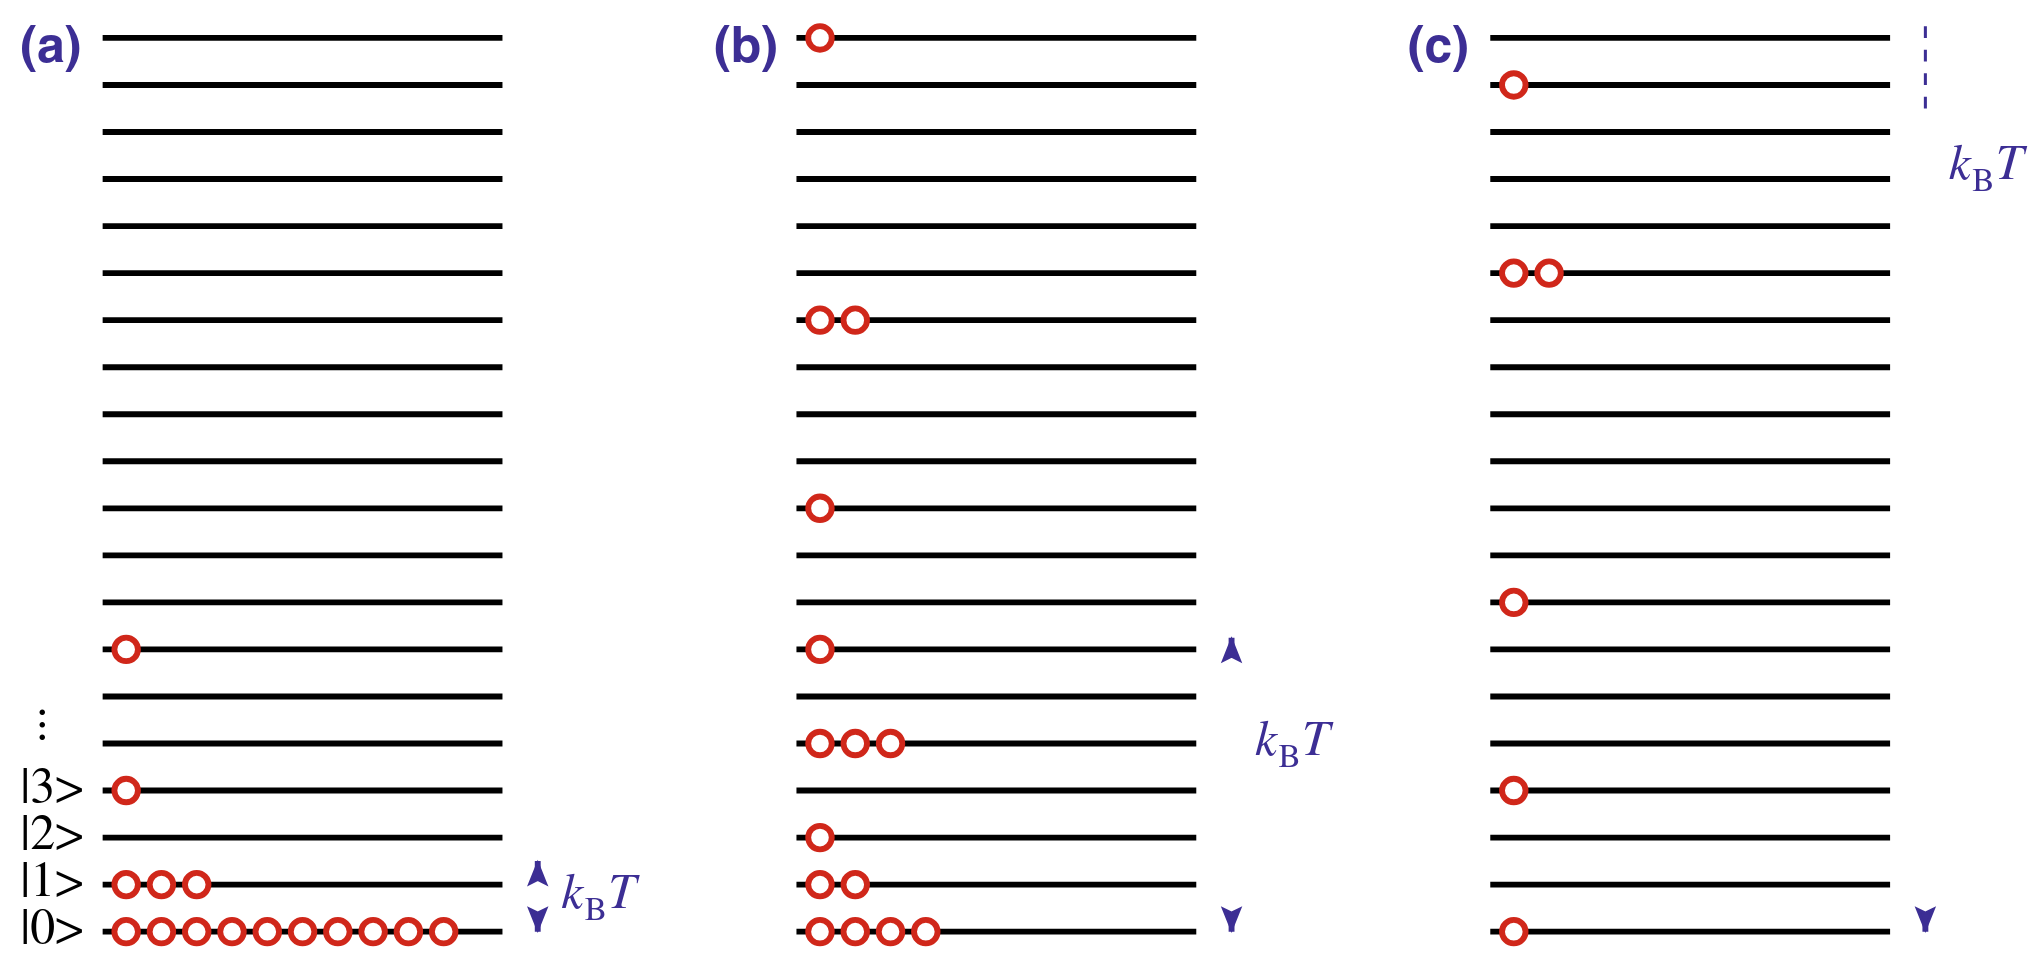
\includegraphics[width = 0.70 \textwidth]{ideal-high-temp.png}
	\caption{Occupancies of single-particle energy eigenstates for a bosonic system in the low-, intermediate- and high-temperature limits.}
	\label{boson-temp}
\end{figure}

\subsection{Limite ad alta temperatura}

Nel limite ad alta temperatura si può non tenere conto dell'occupazione degli stati, poiché il gas si comporta classicamente e $ n_\alpha \in \{0,1\} \,\,\forall \alpha \in \mathcal{I} $. Si ottiene dunque una funzione di partizione ad alta temperatura valida sia per fermioni che per bosoni:
\begin{equation}
	Z \simeq \frac{1}{N!} \sum_{\alpha_1, \dots, \alpha_N \in \mathcal{I}} \exp \left( -\beta \sum_{i = 1}^N E_{\alpha_i} \right) = \frac{1}{N!} \prod_{i = 1}^N Z_i \equiv \frac{Z_1^N}{N!}
\end{equation}
dove $ Z_1 $ è la funzione di partizione single-particle $ Z_1 \equiv \sum_{\alpha \in \mathcal{I}} \exp \left( -\beta E_\alpha \right) $. \\
Essendo in fase gassosa, il centro di massa di ciascuna particella si muove liberamente ed è dunque separabile dai gradi di libertà interni, ovvero $ \mathcal{H}_i = \mathcal{H}_{i,\text{tr}} + \mathcal{H}_{i,\text{int}} $ e $ Z_1 = Z_{1,\text{tr}} Z_{1,\text{int}} $: mentre $ Z_{1,\text{int}} $ dipende dallo specifico spettro di eccitazioni dei gradi di libertà interni, $ Z_{1,\text{tr}} $ è universale e dipende solo dalla massa della particella $ M $ e dal volume in cui si trova il sistema $ V $.

\subsubsection{Gradi di libertà traslazionali}

Si consideri una particella confinata in un cubo macroscopico di volume $ V = L^3 $ e si impongano delle condizioni al contorno periodiche, ovvero che la funzione d'onda sia uguale su facce opposte del cubo. Le autofunzioni $ \psi_\ve{k}(\ve{r}) = L^{-3/2} \exp(i \ve{k} \cdot \ve{r}) $ possono avere solo valori quantizzati di $ \ve{k} $:
\begin{equation*}
	k_j = \frac{2\pi}{L} n_j \,\,,\,\, n_j \in \Z
\end{equation*}
L'energia cinetica traslazionale associata è:
\begin{equation}
	E_\ve{n} = \frac{\hbar^2 \ve{k}^2}{2M} = \frac{(2\pi\hbar)^2}{2M L^2} (n_x^2 + n_y^2 + n_z^2)
\end{equation}
Per $ L $ o $ M $ macroscopicamente grande (limite termodinamico) questo spettro diventa continuo:
\begin{equation*}
	\begin{split}
		Z_{1,\text{tr}}
		& = \sum_{\ve{n} \in \Z^3} e^{-\beta E_\ve{n}} = \sum_{\ve{n} \in \Z^3} \exp \left[ - \beta \frac{(2\pi\hbar)^2}{2M L^2} (n_x^2 + n_y^2 + n_z^2) \right] \\
		& \rightarrow \int_{\R^3} \dd n_x \dd n_y \dd n_z \exp \left[ -\beta \frac{(2\pi\hbar)^2}{2M L^2} (n_x^2 + n_y^2 + n_z^2) \right] = \left( \frac{L}{\hbar} \sqrt{\frac{M k_\text{B} T}{2\pi}} \right)^3
	\end{split}
\end{equation*}
Si può definire la \textit{lunghezza termica}:
\begin{equation}
	\Lambda \defeq \sqrt{\frac{2\pi\hbar^2}{M k_\text{B} T}}
\end{equation}
così da ottenere:
\begin{equation}
	Z_{1,\text{tr}} = \frac{V}{\Lambda^3}
\end{equation}
Si ha dunque:
\begin{equation*}
	Z = \frac{Z_1^N}{N!} = \frac{Z_{1,\text{tr}}^N}{N!} Z_{1,\text{int}}^N \equiv Z_\text{tr} Z_{1,\text{int}}^N
\end{equation*}

\begin{proposition}[before upper = {\tcbtitle}]{Energia interna traslazionale}{}
	\begin{equation}
		U_\text{tr} = \frac{3}{2} N k_\text{B} T
	\end{equation}

	\tcblower

	\begin{proof}
		\begin{equation*}
			\begin{split}
				U_\text{tr}
				& = - \frac{\pa}{\pa \beta} \ln Z_\text{tr} = - \frac{\pa}{\pa \beta} \ln \frac{V^N}{N! \Lambda^{3N}} = 3N \frac{\pa}{\pa \beta} \ln \Lambda = 3N \frac{\pa}{\pa \beta} \ln \sqrt{\beta} = \frac{3N}{2\beta} = \frac{3}{2} N k_\text{B} T
			\end{split}
		\end{equation*}
	\end{proof}
\end{proposition}

Ciò è in accordo con l'equipartizione dell'energia di Boltzmann.

\begin{theorem}{Equazione di stato dei gas perfetti}{}
	Per un gas perfetto vale l'equazione di stato:
	\begin{equation}
		P = \frac{N k_\text{B} T}{V}
	\end{equation}

	\tcblower

	\begin{proof}
		Innanzitutto, si trova l'energia libera nel limite ad alta temperatura:
		\begin{equation*}
			F \defeq - \frac{\ln Z}{\beta} \simeq - \frac{1}{\beta} \ln \frac{(Z_1)^N}{N!} = - \frac{1}{\beta} (N \ln Z_1 - \ln N!) \simeq - \frac{1}{\beta} (N \ln Z_1 - N \ln (N/e))
		\end{equation*}
		dove si è usata l'approssimazione di Stirling $ \ln N! \simeq N \ln (N/e) $. Dunque:
		\begin{equation}
			F = - N k_\text{B} T \ln \frac{e Z_1}{N}
		\end{equation}
		Per la pressione:
		\begin{equation*}
			\begin{split}
				P \defeq - \frac{\pa F}{\pa V} \bigg\vert_{T,N}
				& = - \frac{\pa}{\pa V} \bigg\vert_{T,N} \left[ - N k_\text{B} T \ln \frac{e Z_{1,\text{tr}} Z_{1,\text{int}}}{N} \right] = N k_\text{B} T \frac{\pa}{\pa V} \bigg\vert_{T,N} \left[ \ln \frac{eV}{N \Lambda^3} + \ln Z_{1,\text{int}} \right] \\
				& = N k_\text{B} T \frac{\pa}{\pa V}\bigg\vert_{T,N} \ln \frac{eV}{N \Lambda^3} = N k_\text{B} T \frac{1}{V}
			\end{split}
		\end{equation*}
	\end{proof}
\end{theorem}

Confrontando con $ pV = nRT $, essendo $ N = n N_\text{A} $, si trova $ k_\text{B} = R / N_\text{A} $.

\paragraph{Distribuzione energetica}

Per ricavare la distribuzione di Boltzmann delle energie cinetiche è necessario passare da un'integrale sugli stati $ \ve{n} $ ad un'integrale sull'energia $ E $. La densità degli stati nello spazio degli stati è:
\begin{equation}
	g(\ve{k}) = \frac{\dd n_x}{\dd k_x} \frac{\dd n_y}{\dd k_y} \frac{\dd n_z}{\dd k_z} = \frac{L^3}{8\pi^3} \equiv \frac{V}{8\pi^3}
	\label{eq:dens-k}
\end{equation}
Si vede che gli stati sono distribuiti uniformemente. È necessario trovare la densità degli stati nello spazio delle energie tale per cui:
\begin{equation*}
	g(E) \dd E = g(\ve{k}) \dd^3\ve{k} = g(\ve{k}) 4\pi k^2 \dd k
\end{equation*}
Il differenziale $ \dd k $ si ottiene invertendo la relazione di dispersione $ E = E(k) $, che in questo caso dà:
\begin{equation*}
	k = \sqrt{\frac{2M E}{\hbar^2}}
	\quad \Rightarrow \quad
	\dd k = \sqrt{\frac{M}{2\hbar^2 E}} \dd E
\end{equation*}
Si ottiene dunque:
\begin{equation*}
	g(E) \dd E = \frac{V}{8\pi^3} 4 \pi \frac{2M E}{\hbar^2} \sqrt{\frac{M}{2\hbar^2 E}} \dd E = \frac{V M^{3/2}}{\sqrt{2} \pi^2 \hbar^3} \sqrt{E} \dd E
\end{equation*}
ovvero:
\begin{equation}
	g_\text{tr}(E) = \frac{V M^{3/2}}{\sqrt{2} \pi^2 \hbar^3} \sqrt{E}
	\label{eq:en-deg}
\end{equation}
La distribuzione di probabilità che descrive l'energia di una singola particella si può trovare come:
\begin{equation*}
	\frac{\dd P(E)}{\dd E} = g_\text{tr}(E) \frac{e^{- \beta E}}{Z_{1,\text{tr}}} = \frac{V M^{3/2}}{\sqrt{2} \pi^2 \hbar^3} \sqrt{E} \frac{\Lambda^3}{V} e^{-\beta E}
\end{equation*}
Il risultato è indipendente dal volume e dalla massa della particella, ed è dunque universale (a parità di temperatura):
\begin{equation}
	\frac{\dd P(E)}{\dd E} = \frac{2}{\sqrt{\pi}} \beta^{3/2} \sqrt{E} e^{-\beta E}
	\label{eq:maxw-boltz-en}
\end{equation}
Si può ricavare anche una distribuzione delle velocità, trovando che ciascuna componente di $ \ve{v} = \frac{\ve{p}}{M} $ è distribuita gaussianamente come:
\begin{equation*}
	\frac{\dd P(v_j)}{\dd v_j} = \sqrt{\frac{\beta M}{2\pi}} \exp \left( -\beta \frac{M v_j^2}{2} \right)
\end{equation*}
La distribuzione di $ v \equiv \abs{\ve{v}} $ si trova dall'Eq. \ref{eq:maxw-boltz-en}:
\begin{equation*}
	\frac{\dd P(v)}{\dd v} = \frac{\dd P(E)}{\dd E} \frac{\dd E}{\dd v} = M v \frac{\dd P(E)}{\dd E}
\end{equation*}
Sostituendo $ E = \frac{1}{2} M v^2 $ si trova la \textit{distribuzione di Maxwell-Boltzmann}:
\begin{equation}
	\frac{\dd P(v)}{\dd v} = \sqrt{\frac{2 M^3}{\pi (k_\text{B} T)^3}} v^2 \exp \left( - \frac{M}{2 k_\text{B} T} v^2 \right)
\end{equation}

\subsubsection{Gradi di libertà interni}

Per quanto riguarda $ \mathcal{H}_{i,\text{int}} $, si può assumere una separazione netta tra i gradi di libertà rotazionali e quelli vibrazionali (al pari delle molecole), così da poter scrivere $ \mathcal{H}_{i,\text{int}} = \mathcal{H}_{i,\text{vib}} + \mathcal{H}_{i,\text{rot}} $ e dunque $ Z_{1,\text{int}} = Z_{1,\text{vib}} Z_{1,\text{rot}} $.

\paragraph{Componente vibrazionale}

Addottando l'approssimazione armonica, l'Hamiltoniana vibrazionale si riduce a quella di oscillatore armonico $ E_{1,\text{vib}} = \hbar \omega \left( v + \frac{1}{2} \right) $, con $ \omega \defeq\sqrt{\kappa / \mu} $ e $ \kappa \equiv \frac{\pa^2 V_\text{ad}}{\pa R^2}\vert_{R = R_\text{m}} $.

\begin{proposition}{Funzione di partizione vibrazionale}{}
	Definendo $ x \equiv \theta_\text{vib} / T $, si ha:
	\begin{equation}
		Z_{1,\text{vib}} = \frac{1}{2 \sinh(x/2)}
	\end{equation}

	\tcblower

	\begin{proof}
		\begin{equation*}
			Z_{1,\text{vib}} = \sum_{v \in \N_0} \exp \left[ -\beta \hbar \omega \left( v + \frac{1}{2} \right) \right] = \exp \left( - \frac{x}{2} \right) \sum_{v = 0}^\infty \exp \left( -v x \right) = \frac{e^{-x/2}}{1 - e^{-x}} = \frac{1}{2 \sinh(x/2)}
		\end{equation*}
	\end{proof}
\end{proposition}

Dall'Eqq. \ref{eq:int-en-z}-\ref{eq:cal-spec-z} si ricavano:
\begin{equation}
	U_{1,\text{vib}} = \hbar \omega \left( \frac{1}{2} + \frac{1}{e^x - 1} \right)
\end{equation}
\begin{equation}
	c_{V,1,\text{vib}} = k_\text{B} \left[ \frac{x/2}{\sinh(x/2)} \right]^2
\end{equation}
Si ricordi che, in quanto grandezze estensive, $ U_\text{vib} = N U_{1,\text{vib}} $ e $ c_{V,\text{vib}} = N c_{V,1,\text{vib}} $. Gli andamenti di queste quantità sono riportati in Fig. \ref{vib-heat-int}: si vede che $ U_{1,\text{vib}} $ è asintoticamente lineare in $ T $ (come ci si aspetterebbe, contibuendo per $ 2 \cdot \frac{1}{2} k_\text{B} T $ all'energia interna totale), ed anche $ c_{V,1,\text{vib}} $ tende asintoticamente al suo valore classico. Questo comportamente è detto $ \virgolette{scongelamento} $ dei gradi di libertà rotazionali ed avviene una volta superata la soglia $ \theta_\text{vib} \sim 10^3-10^4 \,\text{K} $.

\begin{figure}
	\centering
	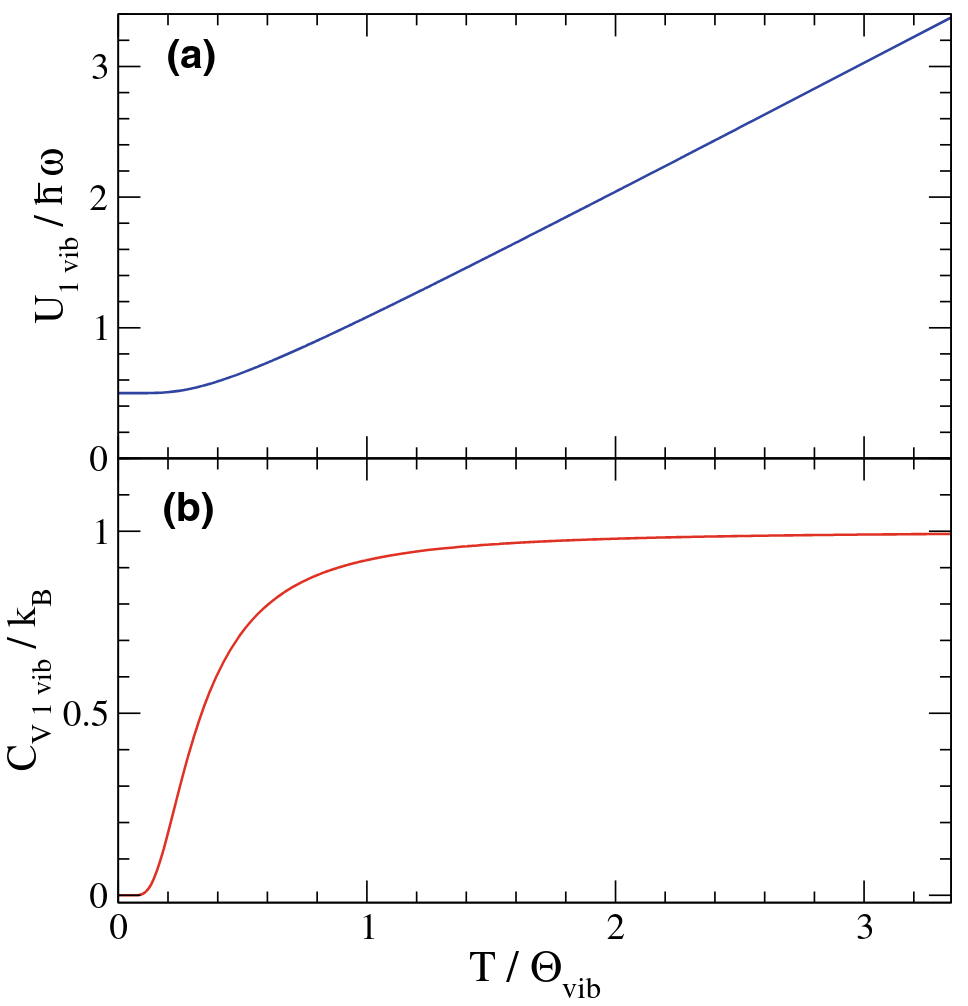
\includegraphics[width = 0.50 \textwidth]{vib-heat-int.png}
	\caption{Temperature dependence of $ U_{1,\text{vib}} $ and $ c_{V,1,\text{vib}} $.}
	\label{vib-heat-int}
\end{figure}

\paragraph{Componente rotazionale}

Nell'approssimazione di rotatore rigido libero, la funzione d'onda rotazionale è un'armonica sferica e lo spettro energetico è $ E_\text{rot} = \frac{\hbar^2}{2I} \ell (\ell + 1) $, con $ I \equiv \mu R_\text{m}^2 $. In questo caso non c'è una forma analitica compatta:
\begin{equation*}
	Z_{1,\text{rot}} = \sum_{\ell \in \N_0} \sum_{m = -\ell}^{\ell} e^{- \frac{\beta \hbar^2}{2I} \ell (\ell + 1)} = \sum_{\ell = 0}^\infty (2\ell + 1) \exp \left[ -\frac{\theta_\text{rot}}{T} \ell (\ell + 1) \right]
\end{equation*}
La temperatura caratteristica $ \theta_\text{rot} $ è tendenzialmente molto bassa ($ \sim 1-10 \,\text{K} $, la più alta è $ 85 \,\text{K} $ per $ \ch{H_2} $), dunque, dato che nel regime $ \theta_\text{rot} / T \ll 1 $ l'esponenziale decade lentamente e molti termini contribuiscono a $ Z_{1,\text{rot}} $, si può approssimare:
\begin{equation*}
	Z_{1,\text{rot}} \simeq \int_0^\infty \dd\ell\, (2\ell + 1) \exp \left[ - \frac{\theta_\text{rot}}{T} \ell (\ell + 1) \right] = \int_0^\infty \dd y\, e^{- \frac{\theta_\text{rot}}{T} y}
\end{equation*}
Si trova quindi che, per $ T \gg \theta_\text{rot} $:
\begin{equation}
	Z_{1,\text{rot}} \simeq \frac{T}{\theta_\text{rot}}
\end{equation}
Dall'Eqq. \ref{eq:int-en-z}-\ref{eq:cal-spec-z} si ricavano:
\begin{equation}
	U_{1,\text{rot}} \simeq k_\text{B} T
\end{equation}
\begin{equation}
	c_{V,1,\text{rot}} \simeq k_\text{B}
\end{equation}
che sono proprio i valori classicamente attesi (confermando il limite ad alta temperatura come il limite classico con $ \virgolette{scongelamento} $ dei gradi di libertà interni). Per $ T \ll \theta_\text{rot} $, invece, l'esponenziale decade velocemente e $ Z_{1,\text{rot}} $ è ottenuto troncando la serie ai primi termini (tendenzialmente si tengono $ \ell = 0 $ e $ \ell = 1 $): l'andamento a tutte le temperature è riportato in Fig. \ref{rot-heat-int}. \\
L'espanzione in serie di $ Z_{1,\text{rot}} $ fornisce anche un metodo quantitativo per calcolare le intensità relative dei picchi di uno spettro roto-vibrazionale, poiché dà la probabilità di occupazione di un livello $ (\ell,m) $ o complessivamente $ \ell $:
\begin{equation}
	P_{\ell,m} = \frac{e^{- \frac{\beta \hbar^2}{2I} \ell (\ell + 1)}}{Z}
	\qquad \qquad
	P_\ell = \frac{2\ell + 1}{Z} e^{- \frac{\theta_\text{rot}}{T} \ell (\ell + 1)}
\end{equation}

\begin{proposition}{}{}
	La riga più intensa in uno spettro roto-vibrazionale è quella associata a $ \ell_\text{max} \rightarrow \ell_\text{max} \pm 1 $, con:
	\begin{equation}
		\ell_\text{max} = \frac{1}{2} \left[ \sqrt{\frac{2T}{\theta_\text{rot}}} - 1 \right]
	\end{equation}

	\tcblower

	\begin{proof}
		La riga più intensa è quella associata al livello rotazionale più popolato. Quest'ultimo si trova ponendo:
		\begin{equation*}
			\frac{\dd P_\ell}{\dd \ell}\bigg\vert_{\ell = \ell_\text{max}} = 0
			\quad \Rightarrow \quad
			2 - (2 \ell_\text{max} + 1)^2 \frac{\theta_\text{rot}}{T} = 0
			\quad \Rightarrow \quad
			\ell_\text{max} = \frac{1}{2} \left[ \sqrt{\frac{2T}{\theta_\text{rot}}} - 1 \right]
		\end{equation*}
	\end{proof}
\end{proposition}

\begin{figure}
	\centering
	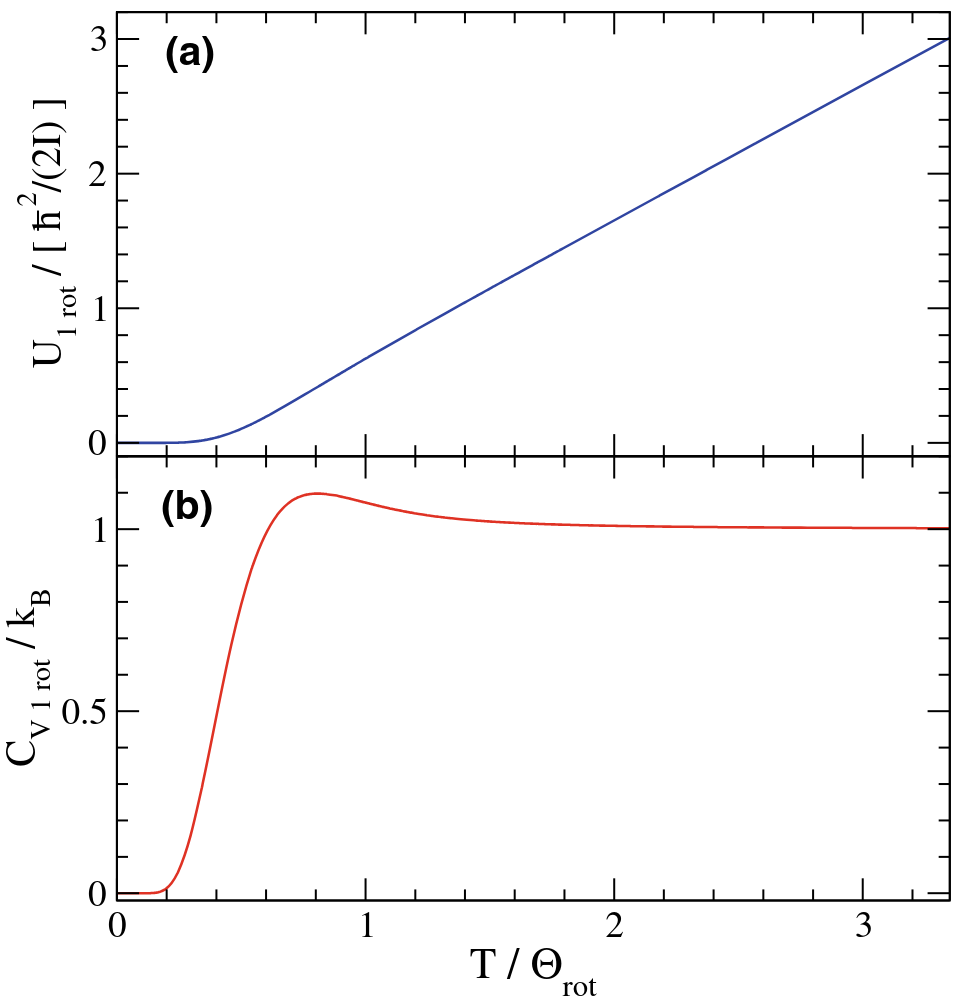
\includegraphics[width = 0.50 \textwidth]{rot-heat-int.png}
	\caption{Temperature dependence of $ U_{1,\text{vib}} $ and $ c_{V,1,\text{vib}} $.}
	\label{rot-heat-int}
\end{figure}

\paragraph{Calore specifico totale}

Mettendo insieme il contributo rotazionale e quello vibrazionale al calore specifico, si ottiene l'andamento in Fig. \ref{vib-rot-c}: a $ T = 0 \,\text{K} $ è presente il solo contributo traslazionale, mentre aumentando la temperatura si scongelano prima i gradi di libertà rotazionali e poi, a temperature sufficientemente elevate, quelli vibrazionali.

\begin{figure}
	\centering
	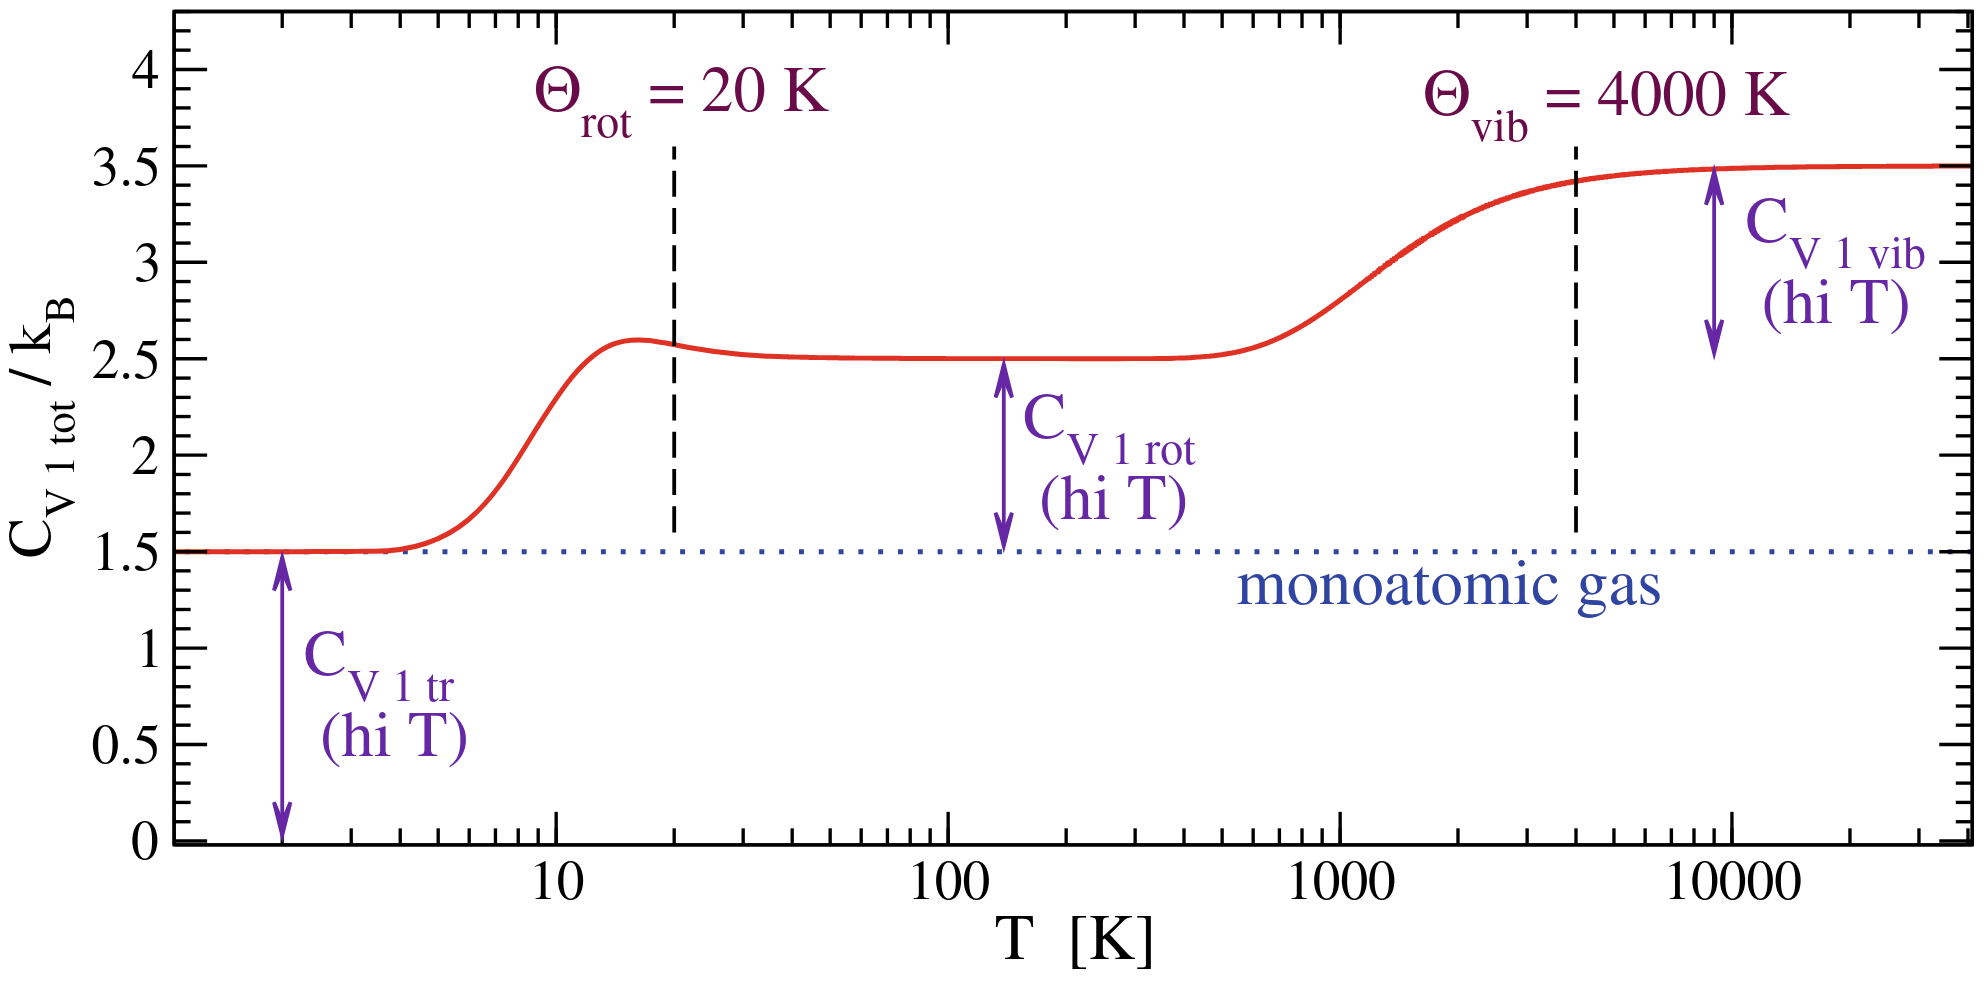
\includegraphics[width = 0.80 \textwidth]{vib-rot-c.png}
	\caption{Temperature dependence of $ c_{V,1} = c_{V,1,\text{tr}} + c_{V,1,\text{rot}} + c_{V,1,\text{vib}} $ for biatomic molecules.}
	\label{vib-rot-c}
\end{figure}

\subsection{Limite a bassa temperatura}

Mentre ad alte temperature sia i sistemi fermionici che quelli bosonici si comportano come dei gas ideali classici, a basse temperature il loro comportamento diverge a causa dei differenti vincoli sull'occupazione dei livelli energetici. \\
Riscrivendo l'Eq. \ref{eq:z-sing-part} rispetto ai numeri d'occupazione (quindi abbandonando la descrizione rispetto alle singole particelle):
\begin{equation}
	Z = \sum_{\alpha_1, \dots, \alpha_N \in \mathcal{I}} \frac{\prod_{k \in \mathcal{I}} n_k!}{N!} \exp \left( -\beta \sum_{i = 1}^N E_{\alpha_i} \right) = \sum_{\{n_\alpha\}} \prod_{\alpha \in \mathcal{I}} \left( e^{-\beta E_\alpha} \right)^{n_\alpha}
	\label{eq:z-n-occ}
\end{equation}
dove $ \{n_\alpha\} \equiv \{n_\alpha \in \mathcal{N}, \alpha \in \mathcal{I} : \sum_{\alpha \in \mathcal{I}} n_\alpha = N\} $, con $ \mathcal{N} = \{0,1\} $ per fermioni e $ \mathcal{N} = \N_0 $ per bosoni. Il vincolo $ \sum_{\alpha \in \mathcal{I}} n_\alpha = N $ rende impossibile dare una forma esplicita a tale sommatoria: per ovviare al problema si introduce un nuovo ensemble, l'\textit{ensemble gran-canonico}, il quale scambia debolmente con l'ambiente non solo energia ma anche particelle. Per mantenere costante e pari a $ N $ il numero medio di particelle, ovvero $ [\hat{N}] = N $, si aggiunge un termine all'autovalore energetico, ottenendo la \textit{funzione di gran-partizione}:
\begin{equation}
	Q \defeq \sum_{N = 0}^\infty \sum_{m(N)} e^{- \beta (E_{m(N)} - \mu N)} \equiv \sum_{N = 0}^\infty \tr e^{- \beta (\mathcal{H} - \mu \hat{N})}
\end{equation}
dove la seconda sommatoria è su tutti gli autostati $ \ket{m(N)} $ di un sistema a $ N $ particelle e $ \mu $ è il potenziale chimico. Essendo $ E_{m(N)} $ una funzione crescente in $ N $, l'esponente $ E_{m(N)} - \mu N $ avrà un minimo per un certo $ N $. Il numero medio di particelle risulta essere:
\begin{equation*}
	[\hat{N}] = \frac{1}{Q} \sum_{N = 0}^\infty \sum_{m(N)} N e^{-\beta (E_{m(N)} - \mu N)} = \frac{1}{\beta} \frac{\pa}{\pa \mu} \ln Q
\end{equation*}

\begin{definition}[before upper = {\tcbtitle}]{Potenziale gran-canonico}{}
	\begin{equation}
		\Omega \defeq - \frac{1}{\beta} \ln Q = - PV
	\end{equation}
\end{definition}

\begin{proposition}{Quantità termodinamiche}{gran-canon-term}
	Si trovano le seguenti relazioni\footnote{L'energia intera si trova da $ U = F + TS $.}:
	\begin{itemize}
		\item numero medio di particelle $ [\hat{N}] = - \frac{\pa \Omega}{\pa \mu}\big\vert_{T,V} $;
		\item entropia $ S = - \frac{\pa \Omega}{\pa T}\big\vert_{\mu,V} $;
		\item energia libera $ F = \Omega + \mu [\hat{N}] $;
		\item potenziale di Gibbs $ G = \mu [\hat{N}] $;
	\end{itemize}
\end{proposition}

Si può calcolare esplicitamente la funzione di gran-partizione per un sistema di bosoni/fermioni non-interagenti.

\begin{theorem}{Gran-partizioni ideali}{}
	Per un sistema di bosoni/fermioni non-interagenti si ha:
	\begin{equation}
		Q = \prod_{\alpha \in \mathcal{I}} \left( 1 - \theta e^{\beta (\mu - E_\alpha)} \right)^{-\theta}
	\end{equation}
	dove $ \theta = +1 $ per sistemi bosonici e $ \theta = -1 $ per sistemi fermionici.

	\tcblower

	\begin{proof}
		Rielaborando l'Eq. \ref{eq:z-n-occ}:
		\begin{equation*}
			\begin{split}
				Q
				& = \sum_{N = 0}^\infty \sum_{\{n_\alpha\}} e^{-\beta ( \sum_{\alpha \in \mathcal{I}} n_\alpha E_\alpha - \mu N)} = \sum_{N = 0}^\infty \sum_{\{n_\alpha\}} e^{-\beta \sum_{\alpha \in \mathcal{I}} n_\alpha (E_\alpha - \mu)} \\
				& = \sum_{n_\alpha \in \mathcal{N}} \prod_{\alpha \in \mathcal{I}} e^{\beta (\mu - E_\alpha) n_\alpha} = \prod_{\alpha \in \mathcal{I}} \sum_{n_\alpha \in \mathcal{N}} \left( e^{\beta (\mu - E_\alpha)} \right)^{n_\alpha}
			\end{split}
		\end{equation*}
		Per fermioni $ \mathcal{N} \equiv \{0,1\} $, quindi:
		\begin{equation*}
			Q = \prod_{\alpha \in \mathcal{I}} \left( 1 + e^{\beta (\mu - E_\alpha)} \right)
		\end{equation*}
		Per bosoni $ \mathcal{N} \equiv \N_0 $, quindi\footnote{Perché la serie geometria coverga, bisogna avere $ \mu - E_\alpha < 0 $, ovvero $ \mu < E_\alpha \,\,\forall \alpha \in \mathcal{I} $. Tipicamente l'energia minima è $ E_\text{min} = 0 $, dunque il potenziale chimico per i bosoni deve essere negativo}:
		\begin{equation*}
			Q = \prod_{\alpha \in \mathcal{I}} \frac{1}{1 - e^{\beta (\mu - E_\alpha)}}
		\end{equation*}
		Definendo il parametro $ \theta $ si ottiene la tesi.
	\end{proof}
\end{theorem}

\begin{theorem}{Statistiche quantistiche}{}
	Per un sistema di bosoni/fermioni non-interagenti si ha:
	\begin{equation}
		[n_\alpha] = \frac{1}{e^{\beta (E_\alpha - \mu)} - \theta}
		\label{eq:fer-dir-bos-ein}
	\end{equation}
	dove $ \theta = +1 $ per sistemi bosonici e $ \theta = -1 $ per sistemi fermionici.

	\tcblower

	\begin{proof}
		Usando la Prop. \ref{prop:gran-canon-term}:
		\begin{equation*}
			\begin{split}
				[\hat{N}]
				& = \frac{1}{\beta} \frac{\pa}{\pa \mu} \ln Q = \frac{1}{\beta} \frac{\pa}{\pa \mu} \sum_{\alpha \in \mathcal{I}} -\theta \ln \left( 1 - \theta e^{\beta (\mu - E_\alpha)} \right) \\
				& = - \frac{\theta}{\beta} \sum_{\alpha \in \mathcal{I}} \frac{-\theta \beta e^{\beta (\mu - E_\alpha)}}{1 - \theta e^{\beta (\mu - E_\alpha)}} = \sum_{\alpha \in \mathcal{I}} \frac{1}{e^{\beta (E_\alpha - \mu)} - \theta}
			\end{split}
		\end{equation*}
		Dato che $ [\hat{N}] = \sum_{\alpha \in \mathcal{I}} [n_\alpha] $ si trova la tesi.
	\end{proof}
\end{theorem}

Queste sono le distribuzioni di Bose-Einstein (bosoni) e Fermi-Dirac (fermioni). Si vede che a $ T $ e $ \mu $ fissati, l'occupazione media di uno stato è determinato esclusivamente dalla sua energia\footnotemark. Inoltre, la presenza di altre particelle influenza l'occupazione media di uno stato tramite il potenziale chimico $ \mu $, il quale è funzione della densità totale media $ [\hat{N}]/V $ e della temperatura $ T $.
%
\footnotetext{In particolare, in assenza di campi magnetici esterni, $ [n_\alpha] $ è indipendente da $ m_s $: di conseguenza, gas ideali di bosoni/fermioni rimangono in uno stato complessivo non-magnetizzato e non-polarizzato a qualsiasi temperatura.}
%
Si noti che giustamente $ [n_\alpha]_\text{Fermi} \in [0,1] $ e che entrambe, per $ E_\alpha \gg \mu $, possono essere approssimate da $ [n_\alpha] \approx e^{-\beta (E_\alpha - \mu)} $, ovvero una distribuzione di Boltzmann (limite classico\footnotemark, opposto al limite degenere a bassa temperatura).

\footnotetext{Considerando un gas perfettamente ideale, ovvero non-interagente, allora se esso venisse preparato in uno stato iniziale lontano dall'equilibrio non raggiungerebbe mai quest'ultimo, in quanto è necessaria un'interazione almeno con l'ambiente.}

\subsubsection{Fermioni}

\begin{figure}
	\centering
	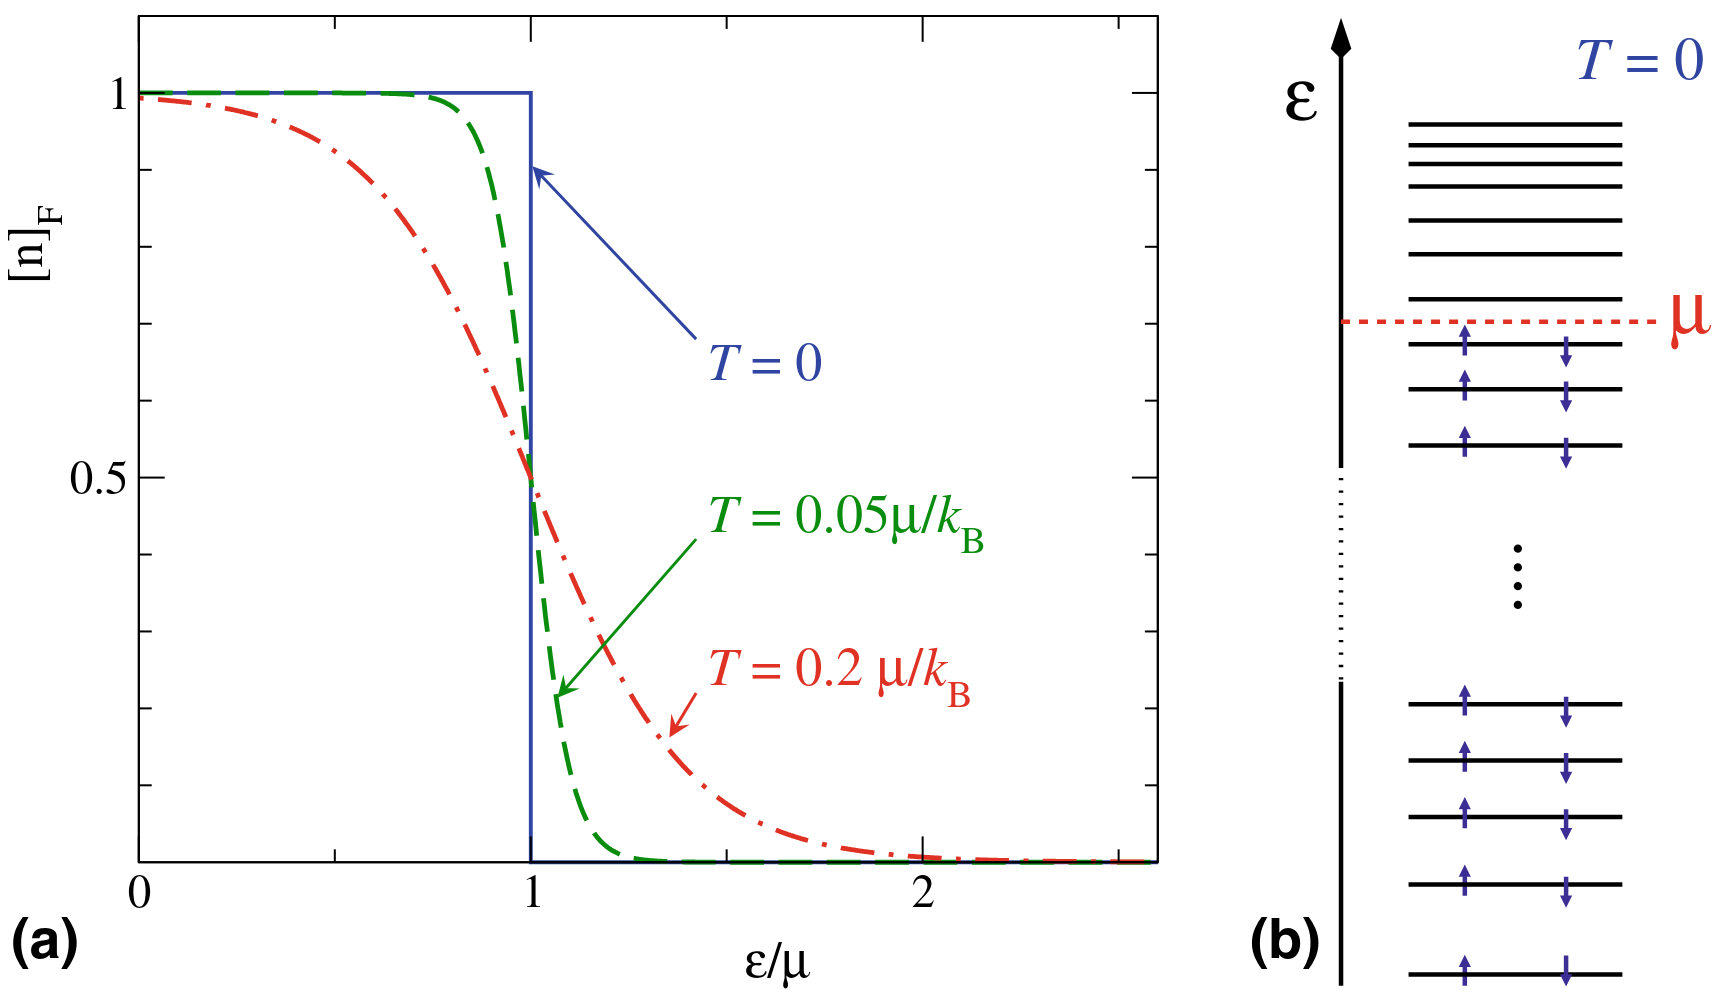
\includegraphics[width = 0.50 \textwidth]{fermi-distr.png}
	\caption{Fermi distribution at various temperatures and filling of single-particle states.}
	\label{fermi-distr}
\end{figure}

Come si vede in Fig. \ref{fermi-distr}, per a $ T = 0 \,\text{K} $ la distribuzione di Fermi-Dirac diventa una funzione a gradino. A questa temperatura, il comportamento del gas di Femi è quello del ground state di un sistema di $ N \equiv [\hat{N}] $ fermioni liberi non-interagenti: questo è ottenuto antisimmetrizzando gli stati in cui vengono riempiti gli $ N $ livelli energetici single-particle con energia più bassa, fino ad un'energia massima $ \varepsilon_\text{F} $ detta \textit{energia di Fermi}.

\begin{theorem}{Energia di Fermi}{}
	L'energia di Fermi è:
	\begin{equation}
		\varepsilon_\text{F} \equiv \mu(T = 0) = \frac{\hbar^2}{2M} \left( \frac{6\pi^2}{g_s} \frac{N}{V} \right)^{2/3}
	\end{equation}
	dove $ g_s $ è la degenerazione da spin dei livelli energetici single-particle.

	\tcblower

	\begin{proof}
		Si noti che, ponendo $ \mu \equiv \mu(T = 0) $:
		\begin{equation*}
			\lim_{T \rightarrow 0} [n_\alpha]_\text{F} =
			\begin{cases}
				1 & E_\alpha < \mu \\
				\frac{1}{2} & E_\alpha = \mu \\
				0 & E_\alpha > \mu
			\end{cases}
		\end{equation*}
		Ricordando l'Eq. \ref{eq:en-deg}:
		\begin{equation*}
			N \equiv [\hat{N}] = \int_0^\infty \dd E\, g(E) [n_\alpha]_\text{F} = \int_0^\mu \dd E\, g(E) = g_s \frac{V M^{3/2}}{\sqrt{2} \pi^2 \hbar^3} \int_0^\mu \dd E\, \sqrt{E} = \frac{(2M)^{3/2} V g_s}{4\pi^2 \hbar^3} \frac{2}{3} \mu^{3/2}
		\end{equation*}
		Risolvendo per $ \mu $ e contando che $ \varepsilon_\text{F} \equiv \mu $ si ha la tesi.
	\end{proof}
\end{theorem}

Passando allo spazio dei momenti, si trova il \textit{momento di Fermi}:
\begin{equation}
	k_\text{F} = \sqrt[3]{\frac{6\pi^2}{g_s} \frac{N}{V}}
	\label{eq:k-f}
\end{equation}
che è concorde con $ N = \frac{4}{3} \pi k_\text{F}^3 \cdot g_s \cdot \frac{V}{8\pi^3} $ (volume $ \cdot $ degenerazione $ \cdot $ densità nello spazio dei momenti).

\begin{example}{Gas di elettroni liberi}{}
	Un esempio di gas di Fermi è l'insieme degli elettroni di conduzione di un metallo, che è un gas di elettroni liberi: per esso $ \frac{N}{V} \sim 10^{29}-10^{30} \,\text{m}^{-3} $, quindi $ k_\text{F} \sim 10^{10} \,\text{m}^{-1} $ ($ v_\text{F} \sim 10^6 \,\text{m}/\text{s} $) e $ \varepsilon_\text{F} \sim 5-10 \ev $.
\end{example}

\begin{proposition}{Energia interna}{}
	A $ T = 0 $ l'energia interna di un gas di Fermi è:
	\begin{equation}
		U(T = 0) = \frac{3}{5} N \varepsilon_\text{F}
	\end{equation}

	\tcblower

	\begin{proof}
		Per calcolo diretto:
		\begin{equation*}
			U(T = 0) = \int_0^\infty \dd E\, E g(E) [n_\alpha]_\text{F} = \int_0^\mu \dd E\, E g(E) = \frac{(2M)^{3/2} V g_s}{4\pi^2 \hbar^3} \frac{2}{5} \varepsilon_\text{F}^{5/2} = \frac{3}{5} N \varepsilon_\text{F}
		\end{equation*}
	\end{proof}
\end{proposition}

Si vede quindi che l'energia interna media per elettrone $ \frac{U}{N} = \frac{3}{5} \varepsilon_\text{F} $ non va a zero per $ T \rightarrow 0 $: questa è una conseguenza del principio di Pauli.

\begin{proposition}{Pressione}{}
	A $ T = 0 $ la pressione di un gas di Fermi è:
	\begin{equation}
		P(T = 0) = \frac{2}{3} \frac{U}{V}
	\end{equation}

	\tcblower

	\begin{proof}
		A $ T = 0 $ si ha $ U = F $, quindi:
		\begin{equation*}
			\begin{split}
				P
				& \defeq - \frac{\pa F}{\pa V}\bigg\vert_{T,\mu} = - \frac{\pa U}{\pa V}\bigg\vert_{T,\mu} = - \frac{\pa}{\pa V}\bigg\vert_{T,\mu} \left[ \frac{(2M)^{3/2} V g_s}{4\pi^2 \hbar^3} \frac{2}{5} \varepsilon_\text{F}^{5/2} \right] \\
				& = - \frac{\pa}{\pa V}\bigg\vert_{T,\mu} \left[ \frac{(2M)^{3/2} V g_s}{4\pi^2 \hbar^3} \frac{2}{5} \left( \frac{\hbar^2}{2M} \right)^{5/2} \left( \frac{6\pi^2}{g_s} \frac{N}{V} \right)^{5/3} \right] \\
				& = \left[ \frac{(2M)^{3/2} g_s}{4\pi^2 \hbar^3} \frac{2}{5} \left( \frac{\hbar^2}{2M} \right)^{5/2} \left( \frac{6\pi^2}{g_s} N \right)^{5/3} \right] \frac{2}{3} V^{-5/3} \\
				& = \left[ \frac{(2M)^{3/2} V g_s}{4\pi^2 \hbar^3} \frac{2}{5} \left( \frac{\hbar^2}{2M} \right)^{5/2} \left( \frac{6\pi^2}{g_s} \frac{N}{V} \right)^{5/3} \right] \frac{2}{3} \frac{1}{V} = \frac{2}{3} \frac{U}{V}
			\end{split}
		\end{equation*}
	\end{proof}
\end{proposition}

Questa relazione è valida in generale: non dipende dalla natura delle particelle (fermioni o bosoni), ma soltanto dall'essere particelle libere in 3 dimensioni, dunque vale per tutti i gas ideali a tutte le temperature, a patto che $ U $ sia puramente cinetica e che la relazione di dispersione sia $ E \propto k^2 $ (bosoni/fermioni con massa non-nulla). \\
Nel caso di un gas classico (non-degenere) si ha $ U = \frac{3}{2} N k_\text{B} T $, ovvero $ P = \frac{N}{V} k_\text{B} T $ (equazione di stato dei gas perfetti). Nel caso non-classico (degenere) si può esprimere la correzione al prim'ordine dell'equazione di stato come:
\begin{equation}
	P \simeq \frac{N}{V} k_\text{B} T \left[ 1 - \theta 2^{-5/2} \delta + o(\delta^2) \right]
\end{equation}
dove si è definito il \textit{parametro di degenerazione}:
\begin{equation}
	\delta \equiv \frac{\Lambda^3 N}{g_s V} = \frac{(2\pi)^{3/2} \hbar^3}{(M k_\text{B} T)^{3/2}} \frac{N}{g_s V}
\end{equation}

\paragraph{Espansione di Sommerfeld}

È possibile estendere l'analisi del gas di Fermi a temperatura finita tramite la cosiddetta \textit{espansione di Sommerfeld}, ovvero trattando perturbativamente in $ T / T_\text{F} $ le quantità che dipendono dalla temperatura: $ T_\text{F} \equiv \varepsilon_\text{F} / k_\text{B} $ è la \textit{temperatura di Fermi} e dà una scala di quando la distribuzione di Fermi si inizia a scostare dalla funzione gradino ($ T_\text{F} \sim 10^4-10^5 \,\text{K} $, dunque a temperatura ambiente si può assumere $ T \approx 0 \,\text{K} $). \\
Si vede innanzitutto che $ \mu = \mu(T) $: poiché variando la temperatura si deve conservare il numero di particelle, ovvero $ \int_0^\infty \dd E\, g(E) [n_\alpha]_\text{F} $, si trova che, perché ciò avvenga, all'aumentare di $ T $ deve diminuire $ \mu(T) $ (il $ \virgolette{centro} $ della distribuzione si deve spostare verso l'origine). L'espansione di Sommerfeld per il potenziale chimico è:
\begin{equation}
	\mu(T) = \varepsilon_\text{F} \left[ 1 - \frac{\pi^2}{12} \left( \frac{T}{T_\text{F}} \right)^2 + \dots \right]
\end{equation}
Per l'energia interna, invece:
\begin{equation}
	U(T) = \frac{3}{5} N \varepsilon_\text{F} \left[ 1 + \frac{5\pi^2}{12} \left( \frac{T}{T_\text{F}} \right)^2 + \dots \right]
\end{equation}
Dato che $ c_V = \frac{\pa U}{\pa T} $, si trova che esso è lineare in $ T $:
\begin{equation}
	C_V(T) = N k_\text{B} \frac{\pi^2}{2} \frac{T}{T_\text{F}} + \dots
\end{equation}
Si noti che, rispetto al valore classico (ad alta temperatura) $ \frac{3}{2} N k_\text{B} $, per $ T \ll T_\text{F} $ questo valore risulta soppresso da $ T / T_\text{F} $: questo è dovuto al fatto che solo i pochi fermioni con energia vicina al potenziale chimico partecipano alle eccitazioni termiche, mentre la maggior parte rimane $ \virgolette{congelata} $ negli livelli energetici più profondi. Inoltre, questo contributo elettronico lineare è presente anche nel calore specifico dei solidi, sebbene sia molto più piccolo dei contributi vibrazionali delle molecole e risulti misurabile solo a basse temperature.

\paragraph{Campi magnetici esterni}

Si consideri un gas di elettroni ($ g_s = 2 $, $ m_s = \pm \frac{1}{2} $). Applicando un campo magnetico WLOG $ \ve{B} = B \hat{\ve{e}}_z $, con $ B > 0 $, si vanno a splittare le energie per elettroni $ \uparrow $ ($ m_s = + \frac{1}{2} $) ed elettroni $ \downarrow $ ($ m_2 = - \frac{1}{2} $). In particolare:
\begin{equation*}
	\mathcal{H}_\text{mag} = - \bs{\mu} \cdot \ve{B} = - \mu_z B = - 2 \mu_\text{B} m_s B = \mp \mu_\text{B} B
\end{equation*}
Si vede dunque che aumenta il numero di elettroni $ \uparrow $ (paralleli a $ \ve{B} $) e diminuisce quello di elettroni $ \downarrow $ (antiparalleli a $ \ve{B} $) il livello energetico con $ m_s = + \frac{1}{2} $ viene splittato in basso rispetto a quello con $ m_s = - \frac{1}{2} $. \\
Questo splitting è molto piccolo ($ \mu_\text{B} \sim 10^{-5} \ev/\text{T} $), ma elimina la degenerazione da spin: $ g_\pm(E) = g(E \mp \mu_\text{B} B)\vert_{g_2 = 1} $. Si ha inoltre $ [\mathcal{H}_\text{mag}] = - [\mu_z] B $, con:
\begin{equation}
	[\mu_z] = -\mu_\text{B} [N_+ - N_-] = \frac{\sqrt[3]{3}}{4\pi^{4/3}} \frac{q_e^2 V}{m_e} \sqrt[3]{\frac{N}{V}} B
\end{equation}
Questo andamento ($ E_\text{mag} \propto B^2 $) è diverso dal caso classico e si parla di \textit{magnetizzazione di Pauli}. Affinché tutti gli elettroni risultino polarizzati $ \uparrow $, bisogna abbassare talmente tanto il livello energetico con $ m_s = + \frac{1}{2} $ da non avere elettroni con $ m_s = - \frac{1}{2} $: la condizione di magnetizzazione totale è dunque $ 2\mu_\text{B} B = \varepsilon_\text{F} $ (splitting energetico).

\subsubsection{Bosoni}

Il ground state di un sistema di $ N $ bosoni è più semplice rispetto a quello di un equivalente fermionico: non valendo alcun principio d'esclusione, tutti i bosoni occupano lo stato di minima energia $ \ket{\ve{k}} = \ket{\ve{0}} $ con $ E_\ve{0} = 0 $; in presenza di una degenerazione da spin $ g_s $, ciascuno stato di spin sarà popolato in media da $ N / g_s $ bosoni. Questo comportamento è confermato dall'Eq. \ref{eq:fer-dir-bos-ein} (con $ \theta = +1 $: per $ T \rightarrow 0 $, $ [n_\alpha] \rightarrow 0 \,\,\forall E_\alpha > \mu $, mentre la singolarità in $ E_\alpha = \mu $ permane. Inoltre, si dimostra che per i bosoni $ \mu = 0 $: infatti, non c'è alcuna legge di conservazione sul numero di bosoni, dunque non c'è alcuna relazione tra l'energia libera ed il numero di particelle del sistema, ovvero $ \mu = \frac{\pa F}{\pa N} = 0 $. \\
Lo spettro energatico di un sistema bosonico è:
\begin{equation}
	E(n_1, n_2, \dots) = \sum_\alpha n_\alpha E_\alpha
\end{equation}
Se comparato con lo spettro di una collezione di oscillatori armonici:
\begin{equation*}
	E(v_1, v_2, \dots) = \sum_\alpha \left( v_\alpha + \frac{1}{2} \right) \hbar \omega_\alpha
\end{equation*}
si vede che questi sono uguali, a meno dell'energia di punto-zero degli oscillatori. In particolare, $ \alpha $ individua o lo specifico oscillatore di pulsazione $ \omega_\alpha $, o lo stato single-particle di energia $ E_\alpha $: l'analogia ha quindi senso, poiché $ v_\alpha \in \N $ e $ n_\alpha \in \N $ (per bosoni). Questa uguaglianza spettrale dà un'analogo comportamento statistico tra i due sistemi: si associa ad ogni eccitazione di un oscillatore armonico una particella (es.: fononi, fotoni, etc.).

\paragraph{Gas di fotoni}

Si può vedere il campo elettromagnetico come un gas di fotoni, ovverosia l'insieme dei modi normali d'oscillazione del campo stesso. Si noti che anche i fotoni hanno $ g_s = 2 $, dato dalle due possibili polarizzazioni circolari. La relazione di dispersione per i fotoni è:
\begin{equation}
	E(\ve{p}) = c \abs{\ve{p}}
	\qquad \Leftrightarrow \qquad
	\omega(\ve{k}) = c \abs{\ve{k}}
\end{equation}
dove il numero d'onda è $ \ve{k} = \frac{\ve{p}}{\hbar} $.

\begin{proposition}{Densità di stati}{}
	La densità di stati di un gas di fotoni è:
	\begin{equation}
		g(E) = \frac{V}{\pi^2 c^3 \hbar^3} E^2
	\end{equation}

	\tcblower

	\begin{proof}
		Dalla relazione di dispersione (assumendo $ V = L^3 $ e condizioni periodiche al contorno):
		\begin{equation*}
			E = c \abs{\ve{p}} = c \hbar \abs{\ve{k}} = c \hbar \frac{2\pi}{L} \abs{\ve{n}}
		\end{equation*}
		Il numero di stati per una data energia è quindi:
		\begin{equation*}
			N = \frac{4}{3} \pi \abs{\ve{n}}^3 = \frac{V E^3}{6 \pi^2 c^3 \hbar^3}
		\end{equation*}
		La densità di stati sarà:
		\begin{equation*}
			\frac{\pa N}{\pa E} = \frac{V}{2 \pi^2 c^3 \hbar^3} E^2
		\end{equation*}
		La tesi si trova contando che $ g(E) = g_s \frac{\pa N}{\pa E} $.
	\end{proof}
\end{proposition}

Si noti che per passare da $ g(E) $ a $ g(\omega) $ o $ g(\nu) $ bisogna imporre $ g(E) \dd E = g(\omega) \dd \omega = g(\nu) \dd \nu $, trovando (con i relativi cambi di misura):
\begin{equation}
	g(\nu) = \frac{8\pi}{c^5} V \nu^2
	\qquad \qquad
	g(\omega) = \frac{V}{\pi^2 c^3} \omega^2
\end{equation}

\begin{theorem}{Densità spettrale (di Planck)}{}
	L'energia interna di un gas di fotoni all'equilibrio in un volume $ V $ a temperatura $ T $ è:
	\begin{equation}
		U = V \int_0^\infty \dd E\, u(E,T) = V \frac{\pi^2 (k_\text{B} T)^4}{15 \hbar^3 c^3}
	\end{equation}
	dove la \textit{densità d'energia spettrale} (o funzione di Planck) è:
	\begin{equation}
		u(E,t) = \frac{1}{\pi^2 c^3 \hbar^3} \frac{E^3}{e^{\beta E} - 1}
	\end{equation}

	\tcblower

	\begin{proof}
		La densità d'energia spettrale è definita come:
		\begin{equation*}
			u(E,T) \defeq \frac{1}{V} g(E) [n_E(T)] E = \frac{1}{\pi^2 c^3 \hbar^3} \frac{E^3}{e^{\beta E} - 1}
		\end{equation*}
		L'energia interna viene quindi espressa come:
		\begin{equation*}
			\begin{split}
				U
				& = \int_0^\infty \dd E\, E g(E) [n_E(T)] = V \int_0^\infty \dd E\, u(E,T) \\
				& = \frac{V}{\pi^2 c^3 \hbar^3} \int_0^\infty \dd E\, \frac{E^3}{e^{\beta E} - 1} = \frac{V}{\pi^2 c^3 \hbar^3} \frac{1}{\beta^4} \int_0^\infty \dd x\, \frac{x^3}{e^x - 1}
			\end{split}
		\end{equation*}
		La tesi si ottiene ricordando che:
		\begin{equation}
			\int_0^\infty \dd x\, \frac{x^3}{e^x - 1} = \frac{\pi^4}{15}
			\label{eq:zeta-3}
		\end{equation}
	\end{proof}
\end{theorem}

La densità d'energia spettrale è più frequentemente trovata in funzione della frequenza:
\begin{equation}
	u(\nu,T) = \frac{8\pi h}{c^3} \frac{\nu^3}{e^{\beta h \nu} - 1}
\end{equation}
Mentre $ u(E,T) $ è una densità d'energia per unità d'energia, dunque ha u.d.m. $ \text{J}/\text{m}^3 \cdot \text{J}^{-1} = \text{m}^{-3} $, $ u(\nu,T) $ è una densità d'energia per unità di frequenza, ovvero ha u.d.m. $ \text{J}/\text{m}^3 \cdot \text{Hz}^{-1} = \text{J}/\text{m}^3 \cdot \text{s} $. \\
La forma della funzione di Planck varia con la temperatura, ma la posizione del suo massimo dipende linearmente da essa. Infatti, imponendo $ \frac{\dd}{\dd \nu} u(\nu, T)\vert_{\nu = \nu_\text{max}} = 0 $ si trova:
\begin{equation*}
	3 \nu_\text{max}^2 (e^{\beta h \nu_\text{max}} - 1) - \nu_\text{max}^3 \beta h e^{\beta h \nu_\text{max}} = 0
	\qquad \Rightarrow \qquad
	x e^x = 3 (e^x - 1)
	\qquad \Rightarrow \qquad
	x \simeq 2.82144\dots
\end{equation*}
dove $ x \equiv \beta h \nu_\text{max} $. Si trova così la \textit{legge di Wien}:
\begin{equation}
	h \nu_\text{max} \simeq 2.82 \cdot k_\text{B} T
\end{equation}

\begin{example}{Misura della temperatura ambientale}{}
	Per $ T = 300 \,\text{K} $ si ha dalla legge di Wien $ \nu_\text{max} \simeq 1.76 \cdot 10^{13} \,\text{Hz} $, ovvero $ h \nu_\text{max} \simeq 71 \,\text{meV} $ (infrarosso): per misurare la temperatura ambientale si può quindi ricorrere alla misura della radiazione infrarossa.
\end{example}

Si noti che parlare di equilibrio termodinamico per un campo elettromagnetico in un volume finito, ad esempio all'interno di una cavità, significa considerare emissione ed assorbimento di fotoni da parte della cavità in modo da mantenerne l'equilibrio termodinamico; nel caso di un volume infinito, invece, si considera un corpo che emette ed assorbe fotoni e che si trova all'equilibrio rispetto all'ambiente. \\
Si consideri per semplicità una cavità di volume finito, definita da una superficie chiusa $ \Sigma $. La potenza netta entrante/uscente dalla cavità è dunque dato dal flusso di energia (trasportata da fotoni) che lo attraversa:
\begin{equation*}
	P(\nu,T) = \int_\Sigma u(\nu,T) \ve{v} \cdot \dd \ve{S} \equiv \int_\Sigma \dd S\, R(\nu,T)
\end{equation*}
dove è stata introdotta la \textit{radianza spettrale}, ovvero una potenza per unità di superficie e di frequenza (u.d.m. $ \text{W}/\text{m}^2 \cdot \text{s} $). Il prodotto scalare determina un fattore $ c \cos \theta $, con $ \theta $ angolo tra la direzione d'incidenza del fotone e la normale alla superficie, il cui valor medio può essere espresso come:
\begin{equation*}
	c \cdot \frac{1}{4\pi} \int_0^{\pi/2} \dd \theta \sin \theta \int_0^{2\pi} \dd \varphi\, \cos \theta = \frac{c}{4}
\end{equation*}
Si trova quindi:
\begin{equation}
	R(\nu,T) = \frac{c}{4} u(\nu,T)
\end{equation}
L'andamento di $ R(E,T) $ è riportato in Fig. \ref{spec-rad}.
Si noti che questa trattazione assume l'assenza di una componente riflessa: tutti i fotoni entranti vengono assorbiti, tutti i fotoni con energia sufficiente vengono emessi. Un corpo (ideale) siffatto è detto \textit{corpo nero}.

\begin{theorem}{Legge di Stefan-Boltzmann}{}
	La \textit{radianza totale} vale:
	\begin{equation}
		R(T) \defeq \int_0^\infty \dd \nu\, R(\nu,T) = \sigma T^4
	\end{equation}
	dove $ \sigma \simeq 5.67 \cdot 10^{-8} \,\text{W}/\text{m}^2 \cdot \text{K}^{-4} $ è la costante di Stefan-Boltzmann.

	\tcblower

	\begin{proof}
		Dalla definizione (ed utilizzando Eq. \ref{eq:zeta-3}):
		\begin{equation*}
			R(T) = \frac{2\pi h}{c^2} \int_0^\infty \dd \nu\, \frac{\nu^3}{e^{\beta h \nu} - 1} = \frac{2\pi h}{c^2} \frac{1}{\beta^4 h^4} \frac{\pi^4}{15} = \frac{2\pi^5}{15 c^2 h^3} k_\text{B}^4 T^4 = \frac{\pi^2 k_\text{B}^4}{60 c^2 \hbar^3} T^4 \equiv \sigma T^4
		\end{equation*}
	\end{proof}
\end{theorem}

\begin{figure}
	\centering
	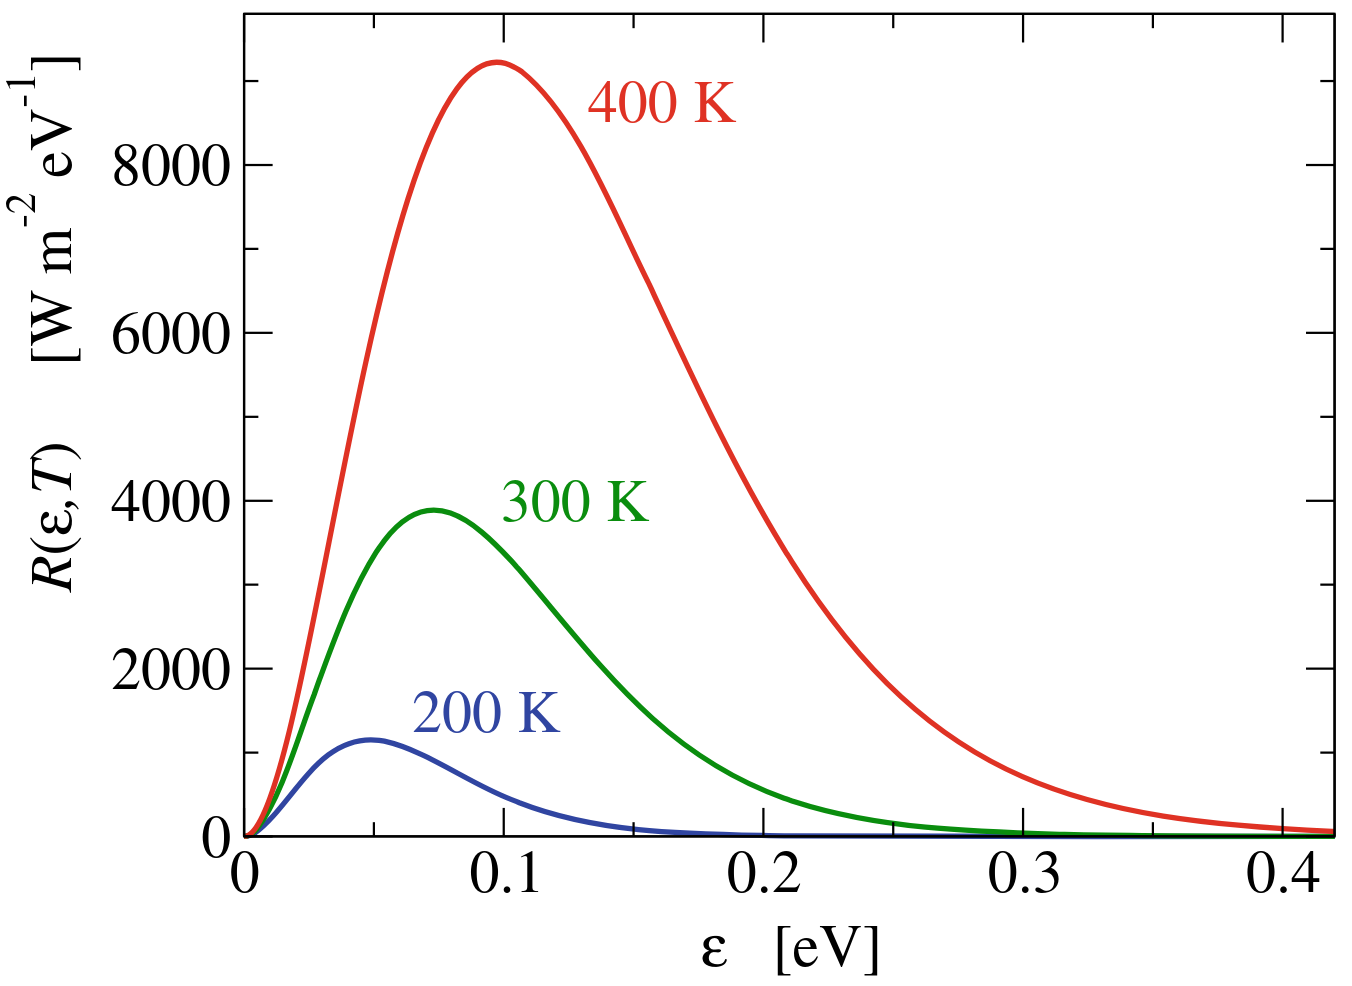
\includegraphics[width = 0.44 \textwidth]{spec-rad.png}
	\caption{Spectral irradiance $ R(E,T) $ of a black body at various temperatures.}
	\label{spec-rad}
\end{figure}

Si può dare consistenza al corpo nero considerando la presenza di radiazione riflessa da parte della sua superficie. Si introduce quindi un coefficiente d'assorbimento $ \alpha(\nu) \in [0,1] $, tale per cui:
\begin{equation}
	R_\text{ass}(\nu,T) = \alpha(\nu) R(\nu,T)
	\qquad \qquad
	R_\text{rif}(\nu,T) = (1 - \alpha(\nu)) R(\nu,T)
\end{equation}
dove $ R(\nu,T) $ è la radianza spettrale incidente. Il corpo nero ha $ \alpha(\nu) \equiv 1 $.

\begin{proposition}{Radianza spettrale emessa}{}
	La radianza spettrale emessa da un corpo non-nero con coefficiente d'assorbimento $ \alpha(\nu) $ è:
	\begin{equation}
		R_\text{em}(\nu,T) = \alpha(\nu) R(\nu,T)
	\end{equation}

	\tcblower

	\begin{proof}
		Dalla conservazione dell'energia $ R(\nu,T) = R_\text{em}(\nu,t) + R_\text{rif}(\nu,T) $, da cui la tesi.
	\end{proof}
\end{proposition}

Si vede dunque che, in generale, $ R_\text{em}(\nu,T) \le R(\nu,T) $, dove l'uguaglianza vale solo per il corpo nero: detta $ R_0(\nu,T) $ la radianza spettrale di corpo nero, si ha $ R_\text{em}(\nu,T) \le R_0(\nu,T) $, dunque non solo i corpi non-neri riflettono parte della radiazione incidente, ma ne emettono anche meno rispetto al corpo nero di uguale temperatura. \\
Tutte queste considerazioni valgono per un sistema all'equilibrio, in cui l'equilibrio termodinamico tra campo elettromagnetico e corpo viene mantenuto dallo scambio di fotoni. Se il corpo viene posto in una regione in cui il campo elettromagnetico è assente, esso perderà energia emettendo fotoni, raffreddandosi di conseguenza: lo spettro di fotoni emessi sarà $ R(\nu,T) = \alpha(\nu) R_0(\nu,T) $, dunque in condizioni di non-equilibrio il corpo nero è quello che si raffredda più velocemente (per irraggiamento); al contrario, il corpo bianco ($ \alpha(\nu) \equiv 0 $) non si raffredderà affatto, in quanto un corpo ideale completamente riflettente non emetterà alcuna radiazione.

\subsection{Interazione radiazione-materia}

Si consideri un ensemble di particelle identiche non-interagenti e, nello spettro single-particle, si considerino soltanto due stati $ \ket{1} , \ket{2} : E_1 < E_2 $. Fotoni risonanti con $ E \approx E_2 - E_1 $ inducono delle transizioni tra questi livelli (si ignorano le transizioni non-risonanti, che avvengono a rate estremamente più bassi). In particolare, la presenza di radiazione induce l'eccitazione $ \ket{1} \rightarrow \ket{2} $ (assorbimento), dunque, definendo la densità d'energia spettrale $ \rho(E) $ (energia per unità di volume ed intervallo spettrale, u.d.m. $ \text{m}^{-3} $), si ha un rate di transizione (u.d.m. $ \text{s}^{-1} $):
\begin{equation}
	R_{1 \rightarrow 2} = B_{12} \rho(E)
\end{equation}
dove $ B_{12} $ è un'opportuna costante dipendente dalle caratteristiche elettro-meccaniche del sistema (si ignorano gli effetti non lineari $ \sim o(\rho^2) $). Per quanto riguarda invece il decadimento $ \ket{2} \rightarrow \ket{1} $ (emissione), esso avviene sia in maniera spontanea che in maniera stimolata, dunque si avrà:
\begin{equation}
	R_{2 \rightarrow 1} = A_{21} + B_{21} \rho(E)
\end{equation}
dove $ B_{21} $ è analoga a $ B_{12} $ ed $ A_{21} $ dà il rate di decadimento spontaneo (in approssimazione di dipolo-elettrico $ A_{21} $ è dato dall'Eq. \ref{eq:electron-trans-prob}). Si noti che, quando un fotone induce un decadimento, il fotone emesso avrà la stessa fase e gli stessi numeri quantici di quello incidente. \\
Queste relazioni valgono indipendentemente dalla condizione del sistema, in quanto i coefficienti dipendono solo dalle sue proprietà microscopiche. In particolare, esse sono valide quando l'ensemble è all'equilibrio rispetto al campo elettromagnetico, nel qual caso $ \rho(E) \equiv u(E,T) $ (funzione di Planck); inoltre, in tale condizione, il numero medio delle particelle nei due stati è uguale, dunque:
\begin{equation}
	[n_1] R_{1 \rightarrow 2} = [n_2] R_{2 \rightarrow 1}
\end{equation}
Inserendo le relative espressioni e risolvendo per $ \rho(E) \equiv u(E,T) $ si trova:
\begin{equation*}
	\frac{\frac{A_{21}}{B_{21}}}{\frac{[n_1]}{[n_2]} \frac{B_{12}}{B_{21}} - 1} = u(E,T) = \frac{1}{\pi^2 c^3 \hbar^3} \frac{E^3}{e^{\beta E} - 1}
\end{equation*}
Dato che all'equilibrio vale la distribuzione di Boltzmann, ovvero $ [n_1] / [n_2] = P_1 / P_2 = e^{\beta (E_2 - E_1)} = e^{\beta E} $, si ottengono così le \textit{relazioni di Einstein}:
\begin{equation}
	B_{12} = B_{21}
	\qquad \qquad
	A_{21} = \frac{E^3}{\pi^2 c^3 \hbar^3} B_{21}
\end{equation}
Ciò conferma le Eqq. \ref{eq:electron-trans-prob}-\ref{eq:stimul-trans-prob}: la prima relazione mostra che il rate stimolato $ \ket{1} \rightarrow \ket{2} $ è uguale a quello $ \ket{2} \rightarrow \ket{1} $, mentre la seconda mostra che, rispetto a quello stimolato, il rate spontaneo ha una dipendenza $ \propto E^3 $.

\subsubsection{Laser}

Le onde elettromagnetiche vengono attenuate quando attraversano un mezzo diverso dal vuoto. Un dispositivo ottico in grado di amplificare la radiazione incidente, piuttosto che ridurla, dovrebbe avere un rate d'emissione superiore a quello d'assorbimento, ovvero:
\begin{equation*}
	\frac{[n_2] R_{2 \rightarrow 1}}{[n_1] R_{1 \rightarrow 2}} = \frac{[n_2]}{[n_1]} \left[ 1 + \frac{A_{21}}{B_{21} \rho(E)} \right] > 1
\end{equation*}
Per un campo elettromagnetico sufficientemente intenso questo rapporto diventa $ [n_2] / [n_1] > 1 $ (infatti $ R_{1 \rightarrow 2} \approx R_{2 \rightarrow 1} $ per campi abbastanza intensi), ovvero un'inversione di popolazione rispetto all'equilibrio $ [n_2] / [n_1] < 1 $. \\
Con un sistema a due livelli non si può avere un laser, in quanto $ 1 < [n_2] / [n_1] = e^{-\beta E} $ implicherebbe $ T < 0 $. Considerando invece un sistema a tre livelli (Fig. \ref{laser}), si devono prendere $ \ket{1},\ket{2},\ket{3} $ tali per cui la transizione $ \ket{1} \rightarrow \ket{3} $, stimolata dal pompaggio ottico, deve essere favorita (elemento di matrice significativamente diverso da 0), $ \ket{3} \rightarrow \ket{2} $ deve essere spontaneamente molto probabile e $ \ket{2} \rightarrow \ket{1} $ deve essere possibile ma poco probabile (ovvero $ \ket{2} $ deve essere uno stato metastabile). In un sistema siffatto è possibile ottenere l'inversione di popolazione $ [n_2] / [n_1] > 1 $. \\
La condizione di metastabilità, che permette di trascurare il decadimento spontaneo $ \ket{2} \rightarrow \ket{1} $, è tanto più difficile da ottenere quanto più è grande $ \Delta E = E_2 - E_1 $, data la dipendenza $ \gamma_{2 \rightarrow 1} \propto \Delta E^3 $: per questo motivo, sono stati prima creati i MASER (Microwave Amplification by Stimulated Emission of Radiation), e solo successivamente i LASER (Light Amplification by Stimulated Emission of Radiation). Si ricordi, infatti, che l'emissione spontanea è per sua natura incoerente, dunque in un laser è necessario avere una dominanza dell'emissione stimolata, che invece è coerente e direzionale\footnote{Dall'equivalenza tra fotoni e oscillatori armonici deriva che l'ampiezza di probabilità per la creazione di un nuovo fotone dipende dall'elemento di matrice dell'operatore di creazione $ \braket{N + 1 | a\dg | N} = \sqrt{N + 1} $ che aumenta all'aumentare di $ N $: nel limite del numero di Avogadro, tale ampiezza tende a $ 1 $, ovvero vengono creati fotoni identici.}.

\begin{figure}
	\centering
	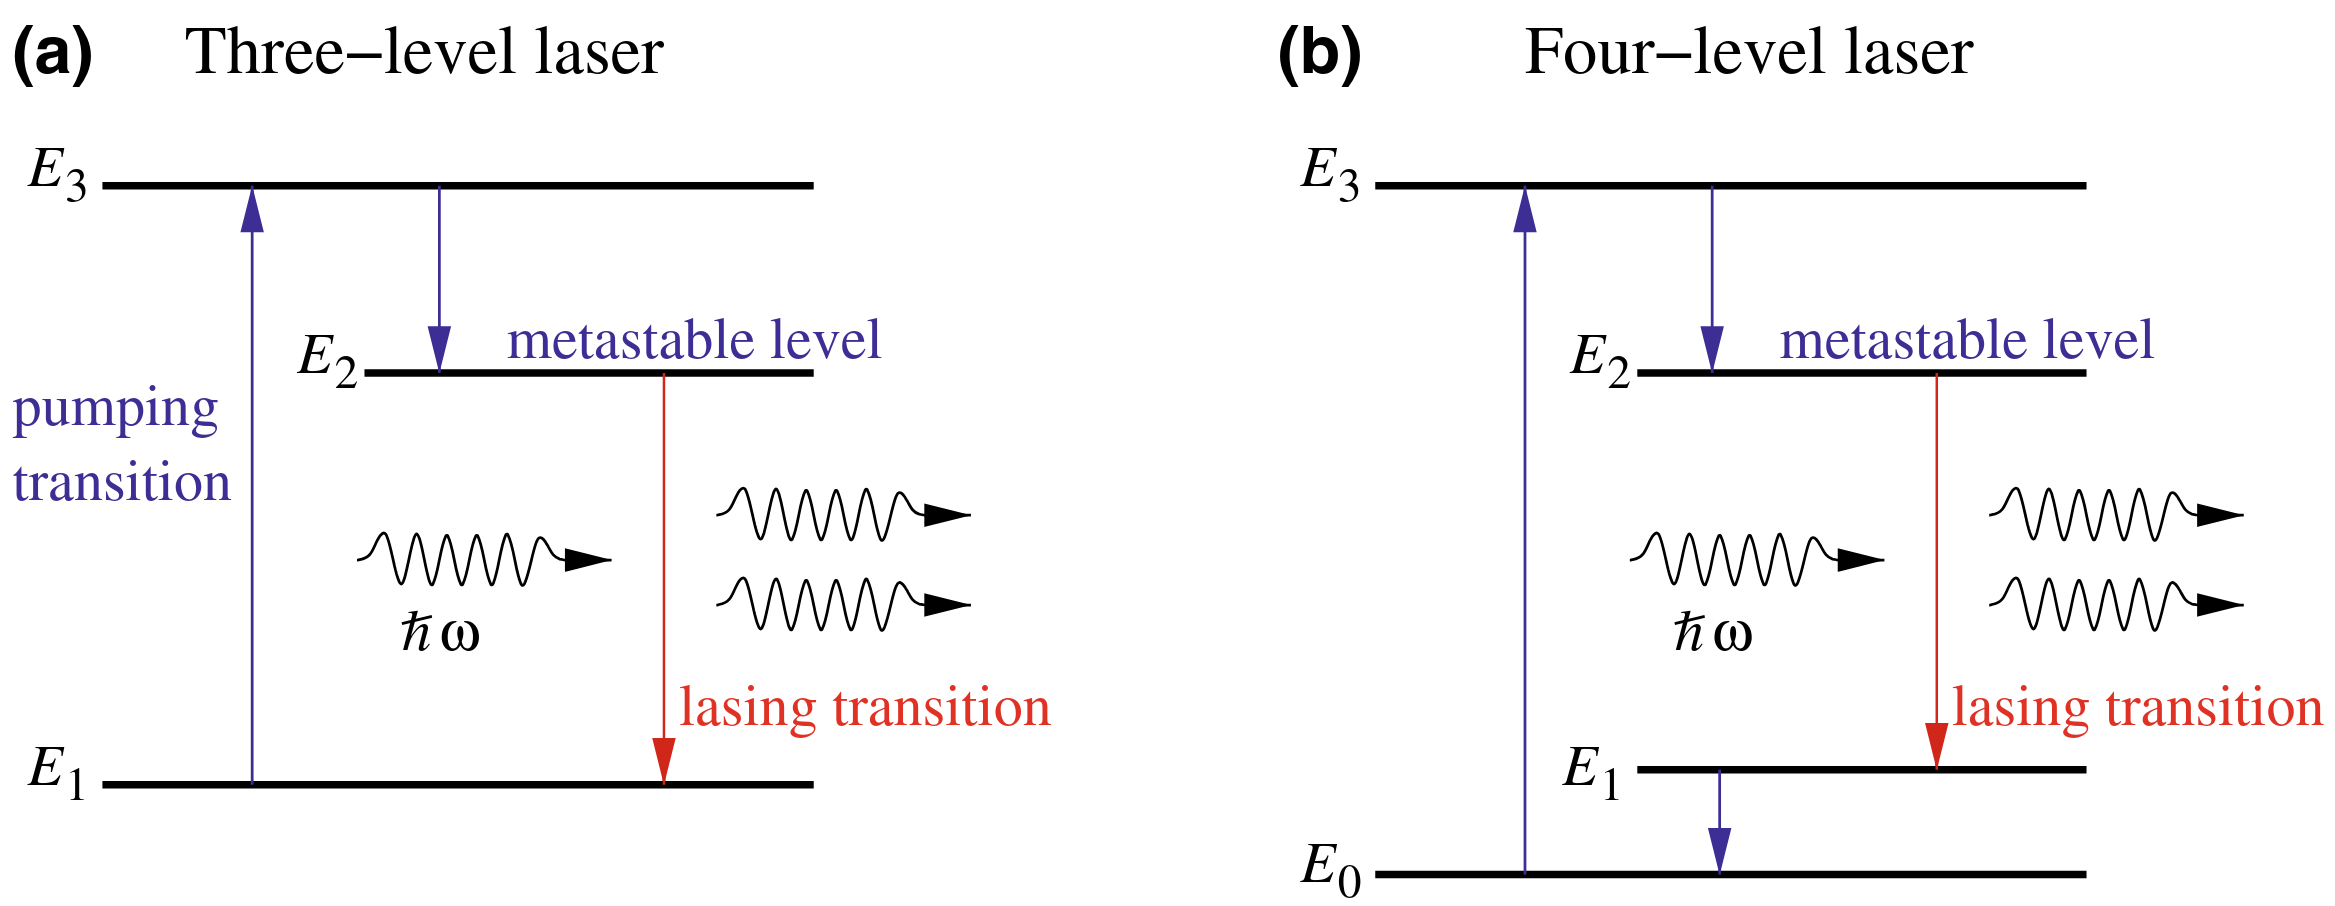
\includegraphics[width = 0.70 \textwidth]{laser.png}
	\caption{Example schemes of lasers.}
	\label{laser}
\end{figure}










